%% abtex2-modelo-trabalho-academico.tex, v-1.9.7 laurocesar
%% Copyright 2012-2018 by abnTeX2 group at http://www.abntex.net.br/ 
%%
%% This work may be distributed and/or modified under the
%% conditions of the LaTeX Project Public License, either version 1.3
%% of this license or (at your option) any later version.
%% The latest version of this license is in
%%   http://www.latex-project.org/lppl.txt
%% and version 1.3 or later is part of all distributions of LaTeX
%% version 2005/12/01 or later.
%%
%% This work has the LPPL maintenance status `maintained'.
%% 
%% The Current Maintainer of this work is the abnTeX2 team, led
%% by Lauro César Araujo. Further information are available on 
%% http://www.abntex.net.br/
%%
%% This work consists of the files abntex2-modelo-trabalho-academico.tex,
%% abntex2-modelo-include-comandos and abntex2-modelo-references.bib
%%
% ------------------------------------------------------------------------
% ------------------------------------------------------------------------
% abnTeX2: Modelo de Trabalho Academico (tese de doutorado, dissertacao de
% mestrado e trabalhos monograficos em geral) em conformidade com 
% ABNT NBR 14724:2011: Informacao e documentacao - Trabalhos academicos -
% Apresentacao
% ------------------------------------------------------------------------
% ------------------------------------------------------------------------
%%
%% Documento ajustado para PCS-EPUSP em 15/mar/2023 por Cintia Borges Margi
% ------------------------------------------------------------------------
%%
\documentclass[
	% -- opções da classe memoir --
	12pt,				% tamanho da fonte
	openright,			% capítulos começam em pág ímpar (insere página vazia caso preciso)
	twoside,			% para impressão em recto e verso. Oposto a oneside
	a4paper,			% tamanho do papel. 
	% -- opções da classe abntex2 --
	%chapter=TITLE,		% títulos de capítulos convertidos em letras maiúsculas
	%section=TITLE,		% títulos de seções convertidos em letras maiúsculas
	%subsection=TITLE,	% títulos de subseções convertidos em letras maiúsculas
	%subsubsection=TITLE,% títulos de subsubseções convertidos em letras maiúsculas
	% -- opções do pacote babel --
	english,			% idioma adicional para hifenização
	french,				% idioma adicional para hifenização
	spanish,			% idioma adicional para hifenização
	brazil				% o último idioma é o principal do documento
	]{abntex2}

% ---
% Pacotes básicos 
% ---
\usepackage{lmodern}			% Usa a fonte Latin Modern			
\usepackage{iftex}
\ifPDFTeX
    \usepackage[T1]{fontenc}
    \usepackage[utf8]{inputenc}
\else
    % Tectonic/XeTeX: fontes Unicode preservam acentos e travessões literais.
    \usepackage{fontspec}
    \defaultfontfeatures{Ligatures=TeX}
    % Nomes de arquivos do pacote TeX: não dependem das fontes do sistema.
    \setmainfont{lmroman12-regular.otf}[
        BoldFont=lmroman12-bold.otf,
        ItalicFont=lmroman12-italic.otf,
        BoldItalicFont=lmroman10-bolditalic.otf]
    \setsansfont{lmsans10-regular.otf}[
        BoldFont=lmsans10-bold.otf,
        ItalicFont=lmsans10-oblique.otf,
        BoldItalicFont=lmsans10-boldoblique.otf]
    \setmonofont{lmmono10-regular.otf}[ItalicFont=lmmono10-italic.otf]
\fi
\usepackage{indentfirst}		% Indenta o primeiro parágrafo de cada seção.
\usepackage{color}				% Controle das cores
\usepackage{graphicx}			% Inclusão de gráficos
\graphicspath{{imagens/}}
\usepackage{microtype} 			% para melhorias de justificação
% ---
		
% ---
% Pacotes adicionais, usados apenas no âmbito do Modelo Canônico do abnteX2
% ---
\usepackage{lipsum}				% para geração de dummy text
% ---

% ---
% Pacotes de citações
% ---
\usepackage[brazilian,hyperpageref]{backref}	 % Paginas com as citações na bibl
\usepackage[alf]{abntex2cite}	% Citações padrão ABNT

%% CBM: pacote para incluir a ficha catalográfica como pdf
\usepackage[final]{pdfpages}

% --- 
% CONFIGURAÇÕES DE PACOTES
% --- 

% ---
% Configurações do pacote backref
% Usado sem a opção hyperpageref de backref
\renewcommand{\backrefpagesname}{Citado na(s) página(s):~}
% Texto padrão antes do número das páginas
\renewcommand{\backref}{}
% Define os textos da citação
\renewcommand*{\backrefalt}[4]{
	\ifcase #1 %
		Nenhuma citação no texto.%
	\or
		Citado na página #2.%
	\else
		Citado #1 vezes nas páginas #2.%
	\fi}%
% ---

% ---
% Informações de dados para CAPA e FOLHA DE ROSTO
% ---
\titulo{FLIKE: desenvolvimento de um protótipo de controle de acesso físico com credenciais temporárias em QR Code e autenticação local}
\autor{Hélcio Prado de Lima, Henrique Eduardo dos Santos de Souza, Mateus Kosicov Perugini}
\local{São Paulo, SP}
\data{2026}
\orientador{Prof. Dr. Reginaldo Arakaki}
\instituicao{%
  Universidade de São Paulo -- USP
  \par
  Escola Politécnica
  \par
  Departamento de Engenharia de Computação e Sistemas Digitais (PCS)}
\tipotrabalho{Monografia de Conclusão de curso (Graduação)}
% O preambulo deve conter o tipo do trabalho, o objetivo, 
% o nome da instituição e a área de concentração 
\preambulo{Trabalho de conclusão de curso apresentado ao Departamento de Engenharia de Computação e Sistemas Digitais da Escola Politécnica da Universidade de São Paulo para obtenção do Título de Engenheiro.}
% ---


% ---
% Configurações de aparência do PDF final

% alterando o aspecto da cor azul
\definecolor{blue}{RGB}{41,5,195}

% informações do PDF
\makeatletter
\hypersetup{
        hypertexnames=false,     % Âncoras únicas mesmo quando a paginação reinicia.
     	%pagebackref=true,
		pdftitle={\@title}, 
		pdfauthor={\@author},
    	pdfsubject={\imprimirpreambulo},
	    pdfcreator={LaTeX with abnTeX2},
		pdfkeywords={FLIKE}{controle de acesso}{QR Code}{AES-CMAC}{ESP32-CAM}{acessibilidade},
		colorlinks=true,       		% false: boxed links; true: colored links
    	linkcolor=blue,          	% color of internal links
    	citecolor=blue,        		% color of links to bibliography
    	filecolor=magenta,      		% color of file links
		urlcolor=blue,
		bookmarksdepth=4
}
\makeatother
% --- 

% ---
% Posiciona figuras e tabelas no topo da página quando adicionadas sozinhas
% em um página em branco. Ver https://github.com/abntex/abntex2/issues/170
\makeatletter
\setlength{\@fptop}{5pt} % Set distance from top of page to first float
\makeatother
% ---

% ---
% Possibilita criação de Quadros e Lista de quadros.
% Ver https://github.com/abntex/abntex2/issues/176
%
\newcommand{\quadroname}{Quadro}
\newcommand{\listofquadrosname}{Lista de quadros}

\newfloat[chapter]{quadro}{loq}{\quadroname}
\newlistof{listofquadros}{loq}{\listofquadrosname}
\newlistentry{quadro}{loq}{0}

% configurações para atender às regras da ABNT
\setfloatadjustment{quadro}{\centering}
\counterwithout{quadro}{chapter}
\renewcommand{\cftquadroname}{\quadroname\space} 
\renewcommand*{\cftquadroaftersnum}{\hfill--\hfill}

\setfloatlocations{quadro}{hbtp} % Ver https://github.com/abntex/abntex2/issues/176
% ---

% --- 
% Espaçamentos entre linhas e parágrafos 
% --- 

% O tamanho do parágrafo é dado por:
\setlength{\parindent}{1.3cm}

% Controle do espaçamento entre um parágrafo e outro:
\setlength{\parskip}{0.2cm}  % tente também \onelineskip

% ---
% compila o indice
% ---
\makeindex
% ---

% ----
% Início do documento
% ----
\begin{document}

% Seleciona o idioma do documento (conforme pacotes do babel)
%\selectlanguage{english}
\selectlanguage{brazil}

% Retira espaço extra obsoleto entre as frases.
\frenchspacing 

% ----------------------------------------------------------
% ELEMENTOS PRÉ-TEXTUAIS
% ----------------------------------------------------------
% \pretextual

% ---
% Capa
% ---
\imprimircapa
% ---

% ---
% Folha de rosto
% (o * indica que haverá a ficha bibliográfica)
% ---
\imprimirfolhaderosto
% ---

% ---
% Inserir a ficha bibliografica
% ---

% Isto é um exemplo de Ficha Catalográfica, ou ``Dados internacionais de
% catalogação-na-publicação''. Você pode utilizar este modelo como referência. 
% Porém, provavelmente a biblioteca da sua universidade lhe fornecerá um PDF
% com a ficha catalográfica definitiva após a defesa do trabalho. Quando estiver
% com o documento, salve-o como PDF no diretório do seu projeto e substitua todo
% o conteúdo de implementação deste arquivo pelo comando abaixo:
%
% A ficha catalográfica definitiva deverá ser inserida depois de emitida pela biblioteca.

% \begin{fichacatalografica}
% 	\sffamily
% 	\vspace*{\fill}					% Posição vertical
% 	\begin{center}					% Minipage Centralizado
% 	\fbox{\begin{minipage}[c][8cm]{13.5cm}		% Largura
% 	\small
% 	\imprimirautor
% 	%Sobrenome, Nome do autor
	
% 	\hspace{0.5cm} \imprimirtitulo  / \imprimirautor. --
% 	\imprimirlocal, \imprimirdata-
	
% 	\hspace{0.5cm} \thelastpage p. : il. (algumas color.) ; 30 cm.\\
	
% 	\hspace{0.5cm} \imprimirorientadorRotulo~\imprimirorientador\\
	
% 	\hspace{0.5cm}
% 	\parbox[t]{\textwidth}{\imprimirtipotrabalho~--~\imprimirinstituicao,
% 	\imprimirdata.}\\
	
% 	\hspace{0.5cm}
% 		1. Palavra-chave1.
% 		2. Palavra-chave2.
% 		3. Palavra-chave3.
% 		I. Orientador.
% 		II. Universidade xxx.
% 		III. Faculdade de xxx.
% 		IV. Título 			
% 	\end{minipage}}
% 	\end{center}
% \end{fichacatalografica}
% ---

% ---
% Inserir errata
% ---
% \begin{errata}
% Elemento opcional da \citeonline[4.2.1.2]{NBR14724:2011}. Exemplo:

% \vspace{\onelineskip}

% FERRIGNO, C. R. A. \textbf{Tratamento de neoplasias ósseas apendiculares com
% reimplantação de enxerto ósseo autólogo autoclavado associado ao plasma
% rico em plaquetas}: estudo crítico na cirurgia de preservação de membro em
% cães. 2011. 128 f. Tese (Livre-Docência) - Faculdade de Medicina Veterinária e
% Zootecnia, Universidade de São Paulo, São Paulo, 2011.

% \begin{table}[htb]
% \center
% \footnotesize
% \begin{tabular}{|p{1.4cm}|p{1cm}|p{3cm}|p{3cm}|}
%   \hline
%    \textbf{Folha} & \textbf{Linha}  & \textbf{Onde se lê}  & \textbf{Leia-se}  \\
%     \hline
%     1 & 10 & auto-conclavo & autoconclavo\\
%    \hline
% \end{tabular}
% \end{table}

% \end{errata}
% ---

% ---
% Inserir folha de aprovação
% ---

% Isto é um exemplo de Folha de aprovação, elemento obrigatório da NBR
% 14724/2011 (seção 4.2.1.3). Você pode utilizar este modelo até a aprovação
% do trabalho. Após isso, substitua todo o conteúdo deste arquivo por uma
% imagem da página assinada pela banca com o comando abaixo:
%
% \begin{folhadeaprovacao}
% \includepdf{folhadeaprovacao_final.pdf}
% \end{folhadeaprovacao}
%
% \begin{folhadeaprovacao}

%   \begin{center}
%     {\ABNTEXchapterfont\large\imprimirautor}

%     \vspace*{\fill}\vspace*{\fill}
%     \begin{center}
%       \ABNTEXchapterfont\bfseries\Large\imprimirtitulo
%     \end{center}
%     \vspace*{\fill}
    
%     \hspace{.45\textwidth}
%     \begin{minipage}{.5\textwidth}
%         \imprimirpreambulo
%     \end{minipage}%
%     \vspace*{\fill}
%    \end{center}
        
%    Trabalho aprovado. \imprimirlocal, 24 de novembro de 2012:

%    \assinatura{\textbf{\imprimirorientador} \\ Orientador} 
%    \assinatura{\textbf{Professor} \\ Convidado 1}
%    \assinatura{\textbf{Professor} \\ Convidado 2}
%    %\assinatura{\textbf{Professor} \\ Convidado 3}
%    %\assinatura{\textbf{Professor} \\ Convidado 4}
      
%    \begin{center}
%     \vspace*{0.5cm}
%     {\large\imprimirlocal}
%     \par
%     {\large\imprimirdata}
%     \vspace*{1cm}
%   \end{center}
  
% \end{folhadeaprovacao}
% ---

% ---
% Dedicatória
% ---
\begin{dedicatoria}
   \vspace*{\fill}
   \centering
   \noindent
   \textit{Este trabalho é dedicado às crianças adultas que,\\
   quando pequenas, sonharam em se tornar cientistas.} \vspace*{\fill}
\end{dedicatoria}
% ---

% ---
% Epígrafe
% ---
% \begin{epigrafe}
%     \vspace*{\fill}
% 	\begin{flushright}
% 		\textit{...}
% 	\end{flushright}
% \end{epigrafe}
% ---

% ---
% RESUMOS
% ---

% resumo em português
\setlength{\absparsep}{18pt} % ajusta o espaçamento dos parágrafos do resumo
\begin{resumo}
Este trabalho apresenta o FLIKE, um protótipo integrado de controle de acesso físico concebido a partir de dificuldades relatadas no acesso à sala de apoio à amamentação e regulação sensorial da Faculdade de Direito da Universidade de São Paulo. O sistema combina uma aplicação web para solicitações e decisões administrativas, uma API e um banco relacional, credenciais temporárias em QR Code e um dispositivo baseado em ESP32-CAM conectado a uma fechadura elétrica. Cada solicitação aprovada produz uma credencial destinada a uma tranca e válida em um intervalo. O payload binário contém identificadores de usuário e tranca e os instantes de emissão e expiração; seus 32 bytes de dados recebem uma tag AES-CMAC de 16 bytes. O frontend codifica o resultado em QR Code versão 3-L. No ponto de acesso, o dispositivo recupera o payload, verifica comprimento, autenticador, destino e intervalo temporal e, diante de uma decisão positiva, comanda um transistor e um relé que acionam a fechadura. Uma demonstração física ponta a ponta confirmou leitura, validação local e atuação sem consulta ao servidor no momento da apresentação. A análise dos 23 requisitos classificou 13 como atendidos, sete como parciais, dois como não atendidos e um como não avaliado. Entre as limitações estão exposição do segredo por rotas da API, impossibilidade de revogação imediata durante a operação local, ausência de sensores de passagem, firmware final não preservado e inexistência de avaliação com usuários. Portanto, o resultado demonstra a viabilidade técnica do protótipo, mas não comprova benefício de acessibilidade nem prontidão para implantação.

\textbf{Palavras-chave}: controle de acesso; QR Code; AES-CMAC; ESP32-CAM; fechadura elétrica; acessibilidade.
\end{resumo}

% resumo em inglês
\begin{resumo}[Abstract]
 \begin{otherlanguage*}{english}
This work presents FLIKE, an integrated physical access control prototype motivated by reported difficulties in accessing the breastfeeding support and sensory regulation room at the University of São Paulo Law School. The system combines a web application for requests and administrative decisions, an API and a relational database, temporary QR Code credentials, and an ESP32-CAM-based device connected to an electric lock. Each approved request produces a credential addressed to one lock and valid within a time interval. Its binary payload contains user and lock identifiers and issue and expiration timestamps; the 32 data bytes receive a 16-byte AES-CMAC tag. The frontend encodes the result as a version 3-L QR Code. At the access point, the device recovers the payload, verifies its length, authenticator, destination, and validity interval, and, after a positive decision, drives a transistor and relay circuit that actuates the lock. An end-to-end physical demonstration confirmed reading, local validation, and actuation without consulting the server when the credential was presented. Of 23 requirements, 13 were classified as satisfied, seven as partially satisfied, two as not satisfied, and one as not evaluated. Limitations include disclosure of the lock secret by API routes, lack of immediate revocation during local operation, absence of passage sensors, failure to preserve the final firmware, and no user evaluation. The result demonstrates the prototype's technical feasibility, but it does not establish accessibility benefits or readiness for deployment.
   \vspace{\onelineskip}
 
   \noindent 
   \textbf{Keywords}: access control; QR Code; AES-CMAC; ESP32-CAM; electric lock; accessibility.
 \end{otherlanguage*}
\end{resumo}

% % resumo em francês 
% \begin{resumo}[Résumé]
%  \begin{otherlanguage*}{french}
%     Il s'agit d'un résumé en français.
 
%    \textbf{Mots-clés}: latex. abntex. publication de textes.
%  \end{otherlanguage*}
% \end{resumo}

% % resumo em espanhol
% \begin{resumo}[Resumen]
%  \begin{otherlanguage*}{spanish}
%    Este es el resumen en español.
  
%    \textbf{Palabras clave}: latex. abntex. publicación de textos.
%  \end{otherlanguage*}
% \end{resumo}
% ---

% ---
% inserir lista de ilustrações
% ---
\pdfbookmark[0]{\listfigurename}{lof}
\listoffigures*
\cleardoublepage
% ---

% ---
% inserir lista de quadros
% ---
\pdfbookmark[0]{\listofquadrosname}{loq}
\listofquadros*
\cleardoublepage
% ---

% ---
% inserir lista de abreviaturas e siglas
% ---
\begin{siglas}
  \item[AES] Advanced Encryption Standard
  \item[API] Application Programming Interface
  \item[CMAC] Cipher-based Message Authentication Code
  \item[GPIO] General-Purpose Input/Output
  \item[HTTP] Hypertext Transfer Protocol
  \item[JSON] JavaScript Object Notation
  \item[JWT] JSON Web Token
  \item[MAC] Message Authentication Code
  \item[QR] Quick Response
  \item[SQL] Structured Query Language
  \item[USP] Universidade de São Paulo
\end{siglas}
% ---

% ---
% inserir o sumario
% ---
\pdfbookmark[0]{\contentsname}{toc}
\tableofcontents*
\cleardoublepage
% ---


% ----------------------------------------------------------
% ELEMENTOS TEXTUAIS
% ----------------------------------------------------------
\textual

% Capítulo 1. Introdução
% Um único .aux para a bibliografia global; as quebras de página são mantidas.
\chapter{Introdução} \label{cap:introducao}

A crescente necessidade de promover acessibilidade, inclusão e autonomia em ambientes institucionais tem impulsionado o desenvolvimento de soluções tecnológicas voltadas ao controle inteligente de acesso a espaços físicos. Em especial, ambientes destinados a públicos com necessidades específicas, como pessoas autistas, neurodivergentes e gestantes, exigem não apenas segurança, mas também processos de acesso que reduzam barreiras sociais, cognitivas e sensoriais.

Nesse contexto, a Faculdade de Direito da Universidade de São Paulo (USP), localizada no histórico prédio do Largo de São Francisco, passou a contar com uma sala de apoio à amamentação e regulação sensorial como parte de suas políticas de inclusão e pertencimento. Apesar de sua importância, o uso desse espaço ainda é limitado por dificuldades relacionadas à segurança e à ausência de um sistema eficiente de controle de acesso. Atualmente, o modelo baseado na retirada manual de chaves junto a funcionários pode gerar constrangimentos, inconsistências de acesso e dificuldades adicionais, especialmente para usuários neurodivergentes.

Diante desse cenário, o projeto CAUSP-LOCK propõe uma solução integrada de hardware e software para viabilizar o acesso seguro, autônomo e simplificado ao ambiente. O sistema utiliza uma fechadura eletrônica baseada em microcontrolador ESP32-CAM e câmera OV2640, capaz de ler e validar QR Codes de acesso gerados por uma aplicação dedicada. Esses códigos são únicos, temporários e protegidos por mecanismos criptográficos, garantindo autenticidade, integridade e irretratabilidade dos acessos, além de permitir a operação offline da tranca.

Além de atender aos requisitos de segurança da informação, o sistema foi projetado com foco em acessibilidade, buscando minimizar a sobrecarga cognitiva e reduzir interações humanas obrigatórias no processo de acesso. Dessa forma, o CAUSP-LOCK se apresenta como uma solução que integra tecnologia, segurança e inclusão, contribuindo para o uso mais eficiente, seguro e digno de espaços institucionais compartilhados.


%%%%%%%%%%%%%%%%%%%%%%%%%%
\section{Motivação}
\begin{itemize}
    \item Subutilização de uma sala inclusiva com alto potencial de impacto social
    \item Dificuldades e constrangimentos no acesso devido ao modelo manual de retirada de chaves
    \item Falta de padronização e critérios claros para concessão de acesso
    \item Vulnerabilidade do espaço a furtos e uso indevido
    \item Necessidade de aliar segurança, acessibilidade e autonomia por meio de tecnologia
\end{itemize}

%%%%%%%%%%%%%%%%%%%%%%%%%%
\section{Objetivo}
\begin{itemize}
    \item Promover o bem-estar de pessoas autistas, neurodivergentes e gestantes
    \item Garantir o uso efetivo da sala de amamentação e regulação sensorial
    \item Reduzir a subutilização do espaço
    \item Aumentar a segurança contra furtos e uso indevido
    \item Eliminar a necessidade de retirada manual de chaves com funcionários
    \item Reduzir constrangimentos no processo de acesso
    \item Padronizar e formalizar o controle de acesso
    \item Permitir acesso autônomo aos usuários autorizados
    \item Implementar autenticação via QR Codes
    \item Garantir segurança por meio de criptografia (autenticidade e integridade)
    \item Utilizar códigos de acesso temporários e de uso único
    \item Possibilitar gestão de acessos via website ou aplicativo
    \item Minimizar esforço e sobrecarga cognitiva dos usuários
    \item Reduzir interações humanas obrigatórias no acesso
    \item Assegurar o uso adequado e controlado do espaço
\end{itemize}

%%%%%%%%%%%%%%%%%%%%%%%%%%
\section{Justificativa}
\begin{itemize}
    \item Necessidade de garantir acesso digno, autônomo e inclusivo a um espaço essencial
    \item Importância de reduzir barreiras enfrentadas por usuários neurodivergentes e gestantes
    \item Demanda por maior segurança e controle no uso de ambientes institucionais
    \item Aplicação de tecnologias acessíveis e de baixo custo para resolver problemas reais
    \item Contribuição para políticas de inclusão e melhoria da experiência dos usuários
\end{itemize}

%%%%%%%%%%%%%%%%%%%%%%%%%%
\section{Organização do Trabalho}
Descrever sucintamente os capítulos e as demais partes do trabalho.

Lembre-se de colocar rótulos nos capítulos e seções (com label{} ) e depois utilizar o ref{}
Por exemplo, o Capítulo \ref{cap:conceitos} apresenta conceitos....
\clearpage

% Capítulo 2. Aspectos Conceituais
\chapter{Aspectos Conceituais} \label{cap:conceitos}

\begin{itemize}
    \item Definir as seções representativas em função do trabalho.
    \item Apresentar os conceitos empregados e a revisão da literatura.
    \item Citar os trabalhos consultados no texto.
\end{itemize}
    
\clearpage

% Capítulo 3. Metodologia do Trabalho
\chapter{Método do trabalho} \label{cap:metodo}

\begin{itemize}
    \item Apresentar o processo de desenvolvimento do trabalho, através das suas fases (por exemplo, especificação de requisitos, projeto, implementação, testes). As fases dependem do tipo do trabalho e devem ser definidas com o apoio do orientador.
    \item O desenvolvimento das fases e seus resultados devem estar descritos nos capítulos seguintes e não no capítulo de Método do Trabalho.
    \item Citar os trabalhos consultados no texto.
\end{itemize}
\clearpage

% Capítulo 4. Especificação de Requisitos
\chapter{Especificação de Requisitos} \label{cap:especificacao}

Este capítulo apresenta os requisitos que delimitam o FLIKE e orientam a análise de seu atendimento. Inicialmente, são descritas a origem dos requisitos, as fronteiras do sistema e as entidades envolvidas. Em seguida, os requisitos são organizados em funcionais, não funcionais e de acessibilidade. Para evitar que uma intenção de projeto seja confundida com um resultado, o estado de atendimento de cada requisito será examinado separadamente, com base em critérios observáveis e nas evidências apresentadas nos capítulos seguintes.

\section{Origem e delimitação dos requisitos}

O problema que motivou o FLIKE foi identificado a partir da experiência de um dos autores, pessoa autista e integrante do Coletivo Autista da USP, de sua participação em uma reunião com dirigentes da Faculdade de Direito da Universidade de São Paulo e de relatos informais de colegas sobre dificuldades para acessar a sala de apoio à amamentação e regulação sensorial. Essas fontes indicaram à equipe um processo dependente da retirada e da liberação de chaves por funcionários, sem um protocolo suficientemente previsível para os potenciais usuários do espaço.

Não foram realizadas entrevistas estruturadas, questionários, observações sistemáticas ou sessões de validação com o público-alvo. Consequentemente, os requisitos apresentados neste capítulo devem ser entendidos como requisitos de projeto definidos pelos autores, e não como necessidades validadas empiricamente junto a pessoas autistas, pessoas neurodivergentes ou usuárias da sala. Em estudo qualitativo com adultos autistas, previsibilidade, disponibilidade antecipada de informações e flexibilidade nos meios de comunicação apareceram entre os fatores relacionados à acessibilidade de espaços públicos \cite{maclennan2023sensory}. Esses resultados fundamentam a direção adotada pela equipe, mas não demonstram que o FLIKE produza os mesmos efeitos. A redução de interações presenciais e a preocupação com estímulos sensoriais orientam o projeto, porém seus efeitos sobre autonomia, constrangimento ou sobrecarga cognitiva não foram medidos.

O catálogo foi consolidado retrospectivamente a partir dos enunciados produzidos no início do trabalho, do protótipo desenvolvido na disciplina Laboratório de Processadores, das decisões tomadas durante a implementação e do comportamento observado nos componentes de software, firmware e hardware. Essa consolidação também incorporou as decisões finais de escopo, como o uso exclusivo de uma aplicação web, a associação da credencial a uma tranca digital e a validação local por AES-CMAC. Propostas abandonadas, como aplicativo móvel, Bluetooth, MQTT, gateway e armazenamento S3, não integram os requisitos finais.

Para tornar os enunciados verificáveis, cada requisito recebe um identificador único e um critério observável. Os requisitos funcionais descrevem comportamentos oferecidos pelo sistema; os não funcionais estabelecem qualidades ou restrições sobre esses comportamentos; e os requisitos de acessibilidade registram critérios técnicos derivados pela equipe. Decisões de implementação, como linguagens, frameworks e modelos de componentes, serão descritas como restrições ou escolhas arquiteturais, sem serem convertidas automaticamente em requisitos.

\section{Escopo e fronteiras do sistema}

O FLIKE abrange o cadastro e a autenticação de usuários; a representação de instituições, edifícios, salas e trancas; a solicitação e a decisão de acesso; a emissão e a apresentação de credenciais digitais em QR Code; a validação local da credencial por um dispositivo baseado em ESP32-CAM; e o acionamento de uma fechadura elétrica. O sistema também contempla consultas administrativas sobre solicitações, credenciais emitidas e seus portadores.

A administração é contextual. Qualquer usuário autenticado pode ser responsável pelas instituições das quais é proprietário e, simultaneamente, solicitar acesso a instituições pertencentes a outras pessoas. Não existe uma classe distinta de cliente, um papel global de administrador, um superadministrador ou, no modelo implementado, a associação de vários responsáveis à mesma instituição.

A aplicação web e a API dependem de conectividade para cadastro, autenticação, gestão, solicitação, decisão e obtenção inicial da credencial. A operação local refere-se ao momento em que a credencial já emitida é apresentada à tranca: a ESP32-CAM deve avaliá-la e comandar o circuito sem consultar o servidor. Arquiteturas nas quais a tranca não mantém comunicação direta com o servidor apresentam um compromisso entre disponibilidade local e consistência do estado de autorização, inclusive diante de revogações \cite{ho2016smartlocks}. No FLIKE, essa escolha implica aceitar a impossibilidade de revogar com confiabilidade uma credencial ainda válida quando o dispositivo não recebe atualizações do servidor.

Não fazem parte do escopo final um aplicativo móvel, a implantação operacional na Faculdade de Direito, a configuração ou a rotação do segredo pelo usuário, a comprovação de entrada, saída ou ocupação da sala e a avaliação de impacto junto ao público-alvo. O CMAC oferece autenticação da origem e integridade de uma mensagem sob a premissa de que o segredo simétrico compartilhado permaneça protegido \cite{nist2005cmac,barker2020keymanagement}; a representação dessa mensagem em QR Code, contudo, pode ser copiada ou redistribuída \cite{kieseberg2010qrcode}. Assim, a credencial registra uma autorização para determinada tranca e janela de validade, mas sua apresentação e o acionamento elétrico não comprovam, isoladamente, qual pessoa física apresentou o código, abriu a porta ou entrou no ambiente.

\section{Atores e entidades do domínio}

Os termos empregados para os atores indicam responsabilidades no sistema e não categorias permanentes de pessoas. Um mesmo usuário pode atuar como solicitante em uma instituição e como responsável em outra. O termo ``administrador'' poderá aparecer ao reproduzir rótulos da interface, mas, no domínio, refere-se ao responsável por uma instituição e não a uma classe separada de conta. O Quadro~\ref{qua:atores-flike} sintetiza esses papéis.

\begin{quadro}[htb]
    \caption{Atores do FLIKE}
    \label{qua:atores-flike}
    \small
    \begin{tabular}{|p{0.27\textwidth}|p{0.63\textwidth}|}
        \hline
        \textbf{Ator} & \textbf{Responsabilidade} \\ \hline
        Usuário & Pessoa cadastrada que autentica uma conta, solicita acesso e consulta as credenciais emitidas para ela. \\ \hline
        Responsável & Usuário que administra uma instituição de sua propriedade, sua estrutura física e as solicitações destinadas às respectivas trancas. \\ \hline
        Fornecedor ou mantenedor & Agente externo que grava previamente no dispositivo o identificador da tranca e o segredo compartilhado. O provisionamento e a rotação desse segredo estão fora do escopo do protótipo. \\ \hline
    \end{tabular}
    \fonte{Elaborado pelos autores.}
\end{quadro}

O Quadro~\ref{qua:entidades-flike} define as entidades centrais empregadas nos requisitos. A distinção entre tranca digital, dispositivo embarcado e fechadura elétrica é necessária porque cada elemento participa de uma etapa diferente da autorização.

\begin{quadro}[htb]
    \caption{Entidades centrais do FLIKE}
    \label{qua:entidades-flike}
    \small
    \begin{tabular}{|p{0.27\textwidth}|p{0.63\textwidth}|}
        \hline
        \textbf{Entidade} & \textbf{Definição} \\ \hline
        Instituição & Entidade organizacional pertencente a um usuário e composta por um ou mais edifícios. \\ \hline
        Edifício & Agrupamento físico pertencente a uma instituição e composto por uma ou mais salas. \\ \hline
        Sala & Espaço físico pertencente a um edifício e associado a uma ou mais trancas digitais. \\ \hline
        Tranca digital & Registro lógico associado a uma sala, a um identificador e a um segredo criptográfico simétrico. \\ \hline
        Dispositivo embarcado & Conjunto constituído por ESP32-CAM, câmera, firmware e interface elétrica, responsável pela leitura e pela decisão local. \\ \hline
        Fechadura elétrica & Atuador físico energizado pelo circuito para permitir o destravamento. \\ \hline
        Solicitação de acesso & Pedido de uma credencial para uma tranca digital, com estado pendente, aprovado ou rejeitado. \\ \hline
        Credencial digital & Payload binário emitido para um usuário e uma tranca, autenticado por AES-CMAC e transportado visualmente por um QR Code. \\ \hline
    \end{tabular}
    \fonte{Elaborado pelos autores.}
\end{quadro}

Neste trabalho, ``chave digital'' é um nome legado da interface para a credencial digital. O termo não deve ser confundido com a chave criptográfica simétrica, que permanece no servidor e no dispositivo, nem com uma chave mecânica. A credencial é emitida uma vez por solicitação aprovada e pode ser reapresentada durante sua janela de validade.

\section{Decisões arquiteturais e restrições de escopo}

As decisões desta seção delimitam uma realização do FLIKE e esclarecem as condições sob as quais os requisitos devem ser interpretados. Elas não transformam automaticamente tecnologias específicas em necessidades do produto: componentes de software, bibliotecas, formatos binários e parâmetros elétricos serão apresentados no Capítulo~\ref{cap:desenvolvimento}, junto de sua implementação.

\subsection{Fronteira entre aplicação conectada e decisão local}

O FLIKE foi concebido como uma aplicação web apoiada por API e banco de dados. Cadastro, autenticação, administração da estrutura física, solicitação, decisão, emissão e obtenção inicial da credencial dependem de conexão. Não foi desenvolvido um aplicativo móvel nativo, nem se exige que a aplicação web continue funcionando sem acesso ao servidor. O usuário pode apresentar o QR Code enquanto o tiver disponível em seu dispositivo, seja diretamente pelo painel conectado, seja por uma cópia previamente salva.

A operação local começa depois da obtenção da credencial. No momento da leitura, o dispositivo embarcado interpreta o QR Code, verifica sua autenticidade e sua validade e decide sobre o acionamento sem consultar a API. Portanto, a expressão ``operação offline'' empregada neste trabalho qualifica a decisão realizada pela tranca, e não o conjunto do sistema.

\subsection{Destino e validade da credencial}

Cada solicitação aprovada produz uma credencial para uma única tranca digital. Quando uma sala possui várias trancas, o pedido deve identificar aquela à qual se destina. Se uma implantação precisar acionar vários dispositivos em conjunto, poderá provisioná-los como uma mesma tranca lógica, com o mesmo identificador e segredo; essa alternativa não altera a existência de um único destino na solicitação e na credencial.

A autorização é temporal: a credencial pode ser reapresentada quantas vezes forem necessárias desde o instante de emissão, inclusive, até o instante de expiração, exclusive. Esse comportamento permite entrar e sair durante o período autorizado e impede que uma credencial antiga volte a ser aceita depois de expirada. O intervalo padrão de 24 horas adotado pela implementação administrativa quando não se informa outra expiração é um parâmetro da versão desenvolvida, e não uma duração universal imposta ao domínio. A codificação binária exata e a distribuição de seus campos serão descritas no Capítulo~\ref{cap:desenvolvimento}.

\subsection{Segredo compartilhado e provisionamento}

O servidor e o dispositivo associado à tranca compartilham um segredo simétrico, usado para calcular e verificar o AES-CMAC da credencial. O protótipo assume que o fornecedor ou mantenedor grave previamente no dispositivo esse segredo e o identificador da tranca correspondente. Configuração pelo usuário, rotação e recuperação do segredo não integram o escopo desenvolvido.

Essa premissa exige proteger o material criptográfico tanto no servidor quanto no dispositivo. Além disso, como o verificador conhece o mesmo segredo que permite gerar uma tag válida, o mecanismo oferece autenticação e integridade sob segredo compartilhado, mas não constitui assinatura digital assimétrica nem produz não repúdio perante terceiros \cite{nist2005cmac,barker2020keymanagement}.

\subsection{Consequências da decisão local}

Uma tranca sem comunicação com o servidor não recebe imediatamente mudanças posteriores à emissão. Assim, o FLIKE não garante a revogação imediata de uma credencial já entregue e ainda válida. O projeto aceita essa limitação e restringe a autorização por meio do instante de expiração autenticado no próprio payload. Reduzir o período de validade diminui a janela de exposição, mas não cria um canal de revogação.

A disponibilidade local também não elimina riscos externos ao procedimento criptográfico. Queda de energia impede o acionamento; perda do aparelho ou cópia do QR Code pode permitir que outra pessoa apresente a credencial; e comprometimento do segredo possibilita produzir tags que o dispositivo reconheça como autênticas. Essas limitações impedem interpretar a aprovação de uma solicitação ou o acionamento da fechadura como comprovação da identidade da pessoa que entrou no espaço.

\subsection{Plataforma física demonstrada}

O protótipo físico integra uma ESP32-CAM e sua câmera a um circuito de acionamento, uma fonte de alimentação e uma fechadura elétrica. Na demonstração de ponta a ponta, o dispositivo leu o QR Code, extraiu a credencial, verificou o AES-CMAC e a validade, emitiu o sinal lógico de abertura, acionou o circuito de potência e destravou a fechadura. A arquitetura, o circuito elétrico, os componentes e os procedimentos empregados nessa demonstração serão documentados no Capítulo~\ref{cap:desenvolvimento}.

O acionamento físico permanece parte do escopo e da contribuição do protótipo. Ele não foi repetido como requisito funcional autônomo porque representa o resultado final do fluxo já definido pelos requisitos de leitura, validação e decisão local.

\subsection{Propostas não incorporadas à solução final}

Aplicativo Flutter, comunicação Bluetooth, MQTT, gateway intermediário e armazenamento S3 apareceram em versões preliminares, mas não integram a arquitetura final. Também permanecem fora do escopo bateria com autonomia especificada, meta de tempo médio entre falhas, compatibilidade universal com fechaduras, registro persistente no dispositivo, sensores de porta, comprovação de entrada ou ocupação e interface para administrar o segredo da tranca. Essas propostas não serão tratadas como funções implementadas nem como compromissos automáticos de trabalho futuro.

\section{Requisitos funcionais}

Os requisitos funcionais descrevem os comportamentos observáveis necessários para realizar o fluxo de controle de acesso. Cada requisito é apresentado por um enunciado normativo, uma justificativa para sua presença no escopo e um critério de verificação. O critério estabelece a evidência esperada, enquanto o estado de atendimento será consolidado posteriormente na matriz de rastreabilidade.

\subsection{Identidade e responsabilidade contextual}

A identidade da conta permite relacionar solicitações e credenciais aos registros do sistema. Essa associação oferece rastreabilidade da conta e da credencial, mas não comprova que a pessoa física titular operou uma sessão ou apresentou o QR Code. A responsabilidade administrativa, por sua vez, decorre da propriedade da instituição e deve ser avaliada em cada operação.

\subsubsection*{RF-01 --- Cadastro e autenticação}

\textbf{Enunciado:} o sistema deve permitir o cadastro e a autenticação de usuários.

\textbf{Justificativa:} os fluxos de solicitação, decisão e consulta de credenciais dependem de uma conta identificável e de uma sessão autenticada. O requisito não inclui autenticação federada, autenticação multifator ou recuperação de senha, que não fazem parte do escopo final.

\textbf{Critério de verificação:} cadastrar uma conta com dados válidos; autenticar essa conta com as credenciais corretas; obter uma sessão aceita por uma operação protegida; e verificar que credenciais incorretas não produzem uma sessão válida.

\subsubsection*{RF-02 --- Responsabilidade contextual}

\textbf{Enunciado:} um usuário autenticado deve poder administrar as instituições das quais é proprietário e solicitar acesso a instituições pertencentes a outros usuários.

\textbf{Justificativa:} o FLIKE não separa permanentemente clientes e administradores. A mesma pessoa pode decidir solicitações no contexto de uma instituição própria e atuar como solicitante em outro contexto. A autorização administrativa deve, portanto, ser derivada da propriedade do recurso acessado.

\textbf{Critério de verificação:} utilizar duas contas e duas instituições para confirmar que cada usuário administra somente a estrutura sob sua propriedade, não consegue modificar a instituição alheia e consegue criar uma solicitação destinada a uma tranca pertencente à outra instituição.

\subsection{Cadastro da estrutura institucional}

A representação hierárquica da estrutura física permite determinar a instituição responsável por uma solicitação e a tranca à qual uma credencial se destina. O cadastro da tranca digital também estabelece o identificador empregado no payload e o segredo necessário à autenticação local.

\subsubsection*{RF-03 --- Gestão de instituições, edifícios, salas e trancas}

\textbf{Enunciado:} o responsável deve poder cadastrar e administrar instituições, edifícios, salas e trancas digitais em uma hierarquia coerente.

\textbf{Justificativa:} solicitações e credenciais precisam ser associadas a recursos físicos identificáveis e ao responsável autorizado a decidir sobre eles. A hierarquia instituição--edifício--sala--tranca fornece essa associação sem atribuir a administração a um papel global.

\textbf{Critério de verificação:} criar, consultar, alterar e excluir recursos em cada nível da hierarquia; verificar a preservação dos vínculos entre os níveis; rejeitar operações executadas por usuário que não seja proprietário da instituição; e impedir exclusões que violem relações ainda existentes.

\subsection{Solicitação e decisão de acesso}

O FLIKE representa a obtenção de acesso como um fluxo explícito: o usuário seleciona a tranca, registra uma solicitação, acompanha seu estado e aguarda a decisão do responsável pela instituição. Essa organização foi concebida pela equipe para aumentar a previsibilidade do processo e reduzir a necessidade de negociação presencial no momento da entrada. A decisão é coerente com relatos de adultos autistas sobre a importância de informações antecipadas e de alternativas à comunicação falada em espaços públicos \cite{maclennan2023sensory}. Entretanto, como não houve avaliação com usuários do FLIKE, essa relação constitui uma justificativa de projeto, e não evidência de benefício produzido pelo protótipo.

\subsubsection*{RF-04 --- Identificação da tranca destinatária}

\textbf{Enunciado:} toda solicitação de acesso deve identificar exatamente uma tranca digital destinatária.

\textbf{Justificativa:} a credencial é autenticada para uma tranca, e não genericamente para uma sala. A identificação explícita evita que o sistema escolha silenciosamente um atuador quando uma sala possuir mais de uma tranca.

\textbf{Critério de verificação:} criar uma solicitação e confirmar o identificador da tranca selecionada; em uma sala com várias trancas, exigir a escolha explícita e verificar que a solicitação preserva essa escolha.

\subsubsection*{RF-05 --- Solicitação e acompanhamento}

\textbf{Enunciado:} o usuário autenticado deve poder solicitar uma credencial para uma tranca e acompanhar o estado \texttt{pending}, \texttt{approved} ou \texttt{rejected} da solicitação.

\textbf{Justificativa:} o estado torna visível se o pedido aguarda decisão, foi aceito ou foi recusado. A consulta deve estar disponível ao solicitante e não pressupõe que a aprovação seja automática.

\textbf{Critério de verificação:} submeter uma solicitação autenticada; consultar o pedido na conta que o criou; observar as três transições previstas; e impedir que outro solicitante altere o estado.

\subsubsection*{RF-06 --- Decisão pelo responsável}

\textbf{Enunciado:} o responsável pela instituição destinatária deve poder consultar e aprovar ou rejeitar solicitações pendentes.

\textbf{Justificativa:} a autorização administrativa pertence ao usuário proprietário da instituição à qual a tranca está vinculada. Um papel global de administrador não faz parte do domínio.

\textbf{Critério de verificação:} confirmar que o proprietário correto visualiza e decide o pedido uma única vez; que um usuário sem propriedade não consegue decidi-lo; e que uma solicitação já decidida não retorna ao estado pendente por repetição da operação.

\subsection{Emissão e apresentação da credencial}

A decisão administrativa e a emissão da credencial são etapas distintas do fluxo. A aprovação deve produzir uma credencial associada ao pedido, ao solicitante e à tranca destinatária, enquanto a rejeição encerra o pedido sem emitir credencial. A política de uma credencial por solicitação não significa uso único: o mesmo QR Code pode ser reapresentado enquanto permanecer dentro de sua janela de validade. A composição e a validação temporal da credencial serão especificadas nos requisitos dedicados ao protocolo e à tranca.

\subsubsection*{RF-07 --- Emissão condicionada à aprovação}

\textbf{Enunciado:} cada solicitação aprovada deve gerar uma credencial digital, enquanto uma solicitação rejeitada não deve gerar credencial.

\textbf{Justificativa:} a credencial materializa a autorização concedida e precisa manter relação inequívoca com o pedido, o usuário e a tranca destinatária.

\textbf{Critério de verificação:} comparar solicitações e credenciais antes e depois de aprovar e rejeitar pedidos; verificar a existência de exatamente uma credencial para a aprovação e nenhuma para a rejeição; e confirmar os vínculos com o solicitante e a tranca.

\subsubsection*{RF-08 --- Consulta e apresentação da credencial}

\textbf{Enunciado:} o usuário deve poder consultar suas credenciais emitidas e apresentar o QR Code correspondente durante a janela de validade.

\textbf{Justificativa:} após a aprovação, o titular precisa recuperar a representação visual utilizada pela tranca. O requisito admite exibição persistente no painel, download para o aparelho ou solução equivalente, desde que a credencial permaneça acessível durante sua vigência. Ele não exige um aplicativo móvel nem implica operação offline da aplicação web.

\textbf{Critério de verificação:} autenticar o solicitante após a aprovação; recuperar a credencial emitida; renderizar o QR Code correto; confirmar sua disponibilidade durante a janela de validade; e impedir que outra conta consulte a credencial sem autorização.

\subsection{Conteúdo e autenticação da credencial}

A credencial digital materializa uma autorização concedida pelo responsável. Sua função é transportar essa autorização do servidor, onde é emitida após a aprovação da solicitação, até a tranca destinatária, que precisa avaliá-la sem consultar a aplicação naquele momento. Para isso, a credencial reúne dados que identificam o sujeito, o destino e o período da autorização e acrescenta um código que permite à tranca verificar localmente sua origem e sua integridade.

\subsubsection*{RF-09 --- Conteúdo da credencial}

\textbf{Enunciado:} cada credencial deve identificar o usuário autorizado e a tranca destinatária e delimitar sua janela de validade por meio dos instantes de emissão e expiração.

\textbf{Justificativa:} esses dados relacionam a autorização ao seu titular lógico, ao atuador correto e ao período em que poderá ser aceita. O identificador do usuário vincula a credencial a uma conta do sistema, mas não comprova a identidade física da pessoa que apresenta o QR Code.

\textbf{Critério de verificação:} emitir uma credencial a partir de uma solicitação aprovada; recuperar seus dados; e confirmar que usuário, tranca, emissão e expiração correspondem à autorização que originou a emissão.

Os dados da autorização, isoladamente, não permitem detectar uma modificação. Um terceiro poderia substituir o usuário, a tranca ou a expiração antes de apresentar o QR Code. Para proteger conjuntamente esses valores, o servidor calcula uma tag AES-CMAC com o segredo simétrico compartilhado com a tranca destinatária. A tranca recalcula a tag sobre os dados recebidos e compara os resultados. O CMAC é um mecanismo de autenticação de mensagens destinado a fornecer garantia de autenticidade e integridade dos dados \cite{nist2005cmac}; ele não cifra o conteúdo da credencial nem constitui uma assinatura digital assimétrica.

\subsubsection*{RF-10 --- Autenticação da credencial}

\textbf{Enunciado:} o sistema deve autenticar conjuntamente todos os dados da credencial com um código verificável localmente pela tranca destinatária.

\textbf{Justificativa:} a tranca precisa detectar credenciais fabricadas e alterações no usuário, na tranca ou na janela temporal sem consultar o servidor. No FLIKE, essa propriedade depende do AES-CMAC e da proteção do segredo compartilhado entre servidor e tranca; qualquer agente que obtenha esse segredo poderá produzir credenciais aceitas como autênticas.

\textbf{Critério de verificação:} emitir uma credencial; validar seu código de autenticação com o segredo da tranca correta; modificar separadamente cada dado protegido sem recalcular o código; e confirmar que todas as versões modificadas falham na autenticação.

Dados da autorização e tag são codificados em uma sequência binária antes da geração do QR Code. Essa representação evita o custo adicional de converter números e bytes arbitrários em texto e reduz a densidade do símbolo apresentado à câmera. A ordem dos campos, a largura de cada valor e a serialização adotada são decisões da implementação e serão detalhadas no Capítulo~\ref{cap:desenvolvimento}.

\subsection{Leitura e validação local}

A câmera captura o QR Code, mas não decide se o acesso está autorizado. O leitor recupera a sequência binária transportada, e o dispositivo interpreta a credencial antes de produzir uma decisão. Essa separação permite distinguir uma leitura bem-sucedida de uma autorização: reconhecer o símbolo não implica que sua estrutura, sua autenticação, seu destino ou sua validade temporal estejam corretos.

\subsubsection*{RF-11 --- Recuperação do payload binário}

\textbf{Enunciado:} o dispositivo embarcado deve ler o QR Code e recuperar integralmente o payload binário da credencial.

\textbf{Justificativa:} a autenticação e a interpretação dos campos dependem de os bytes recebidos serem idênticos aos emitidos. Tratá-los como texto, representação hexadecimal ou cadeia terminada por byte nulo pode alterar ou truncar a credencial.

\textbf{Critério de verificação:} gerar uma credencial que contenha também bytes nulos e valores superiores a \texttt{0x7f}; apresentá-la à câmera; comparar comprimento e conteúdo recuperados no dispositivo com a sequência emitida; e rejeitar símbolos que não forneçam uma credencial completa.

Depois da decodificação, o dispositivo precisa verificar a estrutura recebida, recalcular o código de autenticação, confirmar que a credencial se destina à própria tranca e comparar seu relógio local com os instantes protegidos de emissão e expiração. Essas condições compõem uma única decisão: a falha de qualquer uma delas deve impedir a autorização.

\subsubsection*{RF-12 --- Validação local da credencial}

\textbf{Enunciado:} antes de autorizar o acesso, o dispositivo deve verificar localmente a estrutura da credencial, seu código de autenticação, a identidade da tranca destinatária e sua janela de validade.

\textbf{Justificativa:} uma tag válida permite detectar alterações realizadas sem conhecimento do segredo, mas não basta quando a credencial se destina a outra tranca ou está fora do período autorizado. Todas as condições precisam ser avaliadas localmente antes de uma decisão positiva.

\textbf{Critério de verificação:} apresentar uma credencial válida e, separadamente, casos com estrutura, tag, identificador da tranca, emissão ou expiração inválidos; confirmar que somente o caso integralmente válido produz autorização.

A janela de autorização é fechada no instante de emissão e aberta no instante de expiração: a credencial vale quando o relógio local satisfaz \texttt{issued\_at <= agora < expires\_at}. A apresentação não consome a credencial nem depende de uma flag de uso no servidor. Assim, o usuário pode reapresentar o mesmo QR Code durante o período concedido, mas não antes dele nem a partir de seu término.

\subsubsection*{RF-13 --- Reapresentação durante a janela de autorização}

\textbf{Enunciado:} uma credencial autêntica destinada à tranca deve poder ser reapresentada enquanto estiver em sua janela de autorização e deve ser rejeitada antes da emissão e a partir da expiração.

\textbf{Justificativa:} cada solicitação aprovada produz uma credencial temporária, e não um passe consumível. O usuário pode apresentá-la quantas vezes forem necessárias dentro do período concedido; credenciais antigas não devem autorizar acessos posteriores.

\textbf{Critério de verificação:} apresentar a mesma credencial ao menos duas vezes dentro do intervalo e confirmar duas autorizações; apresentá-la antes da emissão, exatamente na expiração e depois dela; e confirmar a rejeição nos três casos.

\subsection{Consulta administrativa de credenciais}

O histórico administrativo do FLIKE representa credenciais emitidas e autorizações concedidas. Cada registro pode relacionar o usuário titular, a tranca destinatária e os instantes de emissão e expiração. A existência desse registro comprova que o sistema emitiu uma credencial depois da aprovação, mas não demonstra que o QR Code foi apresentado, que a fechadura abriu ou que alguém entrou no ambiente.

\subsubsection*{RF-14 --- Consulta administrativa de credenciais}

\textbf{Enunciado:} o responsável deve poder consultar os usuários que receberam credenciais e o histórico de credenciais emitidas para as trancas das instituições que administra.

\textbf{Justificativa:} a consulta permite acompanhar as autorizações concedidas dentro do escopo administrativo do proprietário sem transformá-las em evidência de acesso físico. O resultado precisa preservar os vínculos entre usuário, tranca e período autorizado.

\textbf{Critério de verificação:} emitir credenciais para trancas pertencentes a duas instituições com proprietários distintos; confirmar que cada responsável consulta somente os registros de sua instituição; verificar usuário, tranca, emissão e expiração; e confirmar que a interface não rotula a emissão como entrada, saída ou ocupação.

\section{Requisitos não funcionais}

Os requisitos não funcionais estabelecem restrições sobre a forma como os comportamentos anteriores devem ser realizados.

\subsubsection*{RNF-01 --- Decisão local sem consulta ao servidor}

\textbf{Enunciado:} a decisão de autorização e o acionamento da fechadura não devem depender de consulta ao servidor no momento da leitura.

\textbf{Justificativa:} a operação local permite avaliar uma credencial já emitida mesmo quando a tranca está sem conectividade. Para isso, identificador, segredo e referência temporal precisam estar disponíveis no dispositivo. Solicitação, aprovação, emissão e obtenção inicial do QR Code continuam dependentes da aplicação web e da API.

\textbf{Critério de verificação:} deixar o dispositivo sem conexão de rede e, com identificador, segredo e relógio disponíveis localmente, apresentar uma credencial válida; confirmar que leitura, validação, decisão e acionamento são concluídos sem comunicação com o servidor.

\subsubsection*{RNF-02 --- Autenticação e autorização administrativa}

\textbf{Enunciado:} operações administrativas e decisões sobre solicitações devem exigir autenticação e respeitar a propriedade da instituição envolvida.

\textbf{Justificativa:} o papel administrativo é contextual. Estar autenticado não autoriza um usuário a administrar instituições de terceiros, e nenhuma operação administrativa sensível deve ser executada anonimamente.

\textbf{Critério de verificação:} para cada operação administrativa e decisão de solicitação, executar chamadas como proprietário, como usuário autenticado sem propriedade e sem autenticação; confirmar sucesso somente para o proprietário correto.

\subsubsection*{RNF-03 --- Não exposição do segredo da tranca}

\textbf{Enunciado:} o segredo AES-CMAC associado a cada tranca não deve ser exposto a usuários, respostas da API ou registros da aplicação.

\textbf{Justificativa:} quem conhece o segredo pode calcular tags aceitas como autênticas pela tranca. O valor deve permanecer restrito ao servidor e ao dispositivo provisionado, conforme a premissa criptográfica do projeto e a necessidade de proteção do material criptográfico durante seu ciclo de vida \cite{barker2020keymanagement}. Esse requisito trata da exposição pelas interfaces do sistema; armazenamento seguro, rotação e provisionamento são decisões arquiteturais próprias.

\textbf{Critério de verificação:} inspecionar respostas de cadastro, consulta e alteração de trancas, mensagens de erro e registros produzidos pela aplicação; confirmar que o segredo não aparece em nenhum desses canais destinados a usuários ou operadores comuns.

\subsubsection*{RNF-04 --- Responsividade da aplicação web}

\textbf{Enunciado:} a aplicação web deve manter suas funções principais utilizáveis em telas representativas de celular e computador, sem perda de conteúdo ou de controles essenciais.

\textbf{Justificativa:} solicitação, acompanhamento, decisão e consulta do QR Code podem ocorrer em dispositivos diferentes. A adaptação do layout deve preservar a execução desses fluxos, sem exigir um aplicativo móvel separado. Responsividade, isoladamente, não demonstra acessibilidade da interface.

\textbf{Critério de verificação:} executar cadastro, autenticação, solicitação, decisão administrativa e consulta da credencial nos viewports definidos para celular e computador; confirmar que textos e controles essenciais permanecem visíveis, acionáveis e sem sobreposição.

Para o transporte óptico da credencial, versão e nível de correção de erros determinam a quantidade de módulos e a capacidade do QR Code; níveis mais altos de correção reservam maior parcela do símbolo para redundância e reduzem o espaço disponível para dados \cite{denso2012qressentials}.

\subsubsection*{RNF-05 --- Compatibilidade óptica do QR Code}

\textbf{Enunciado:} a representação completa da credencial deve ser codificada em modo binário como QR Code versão 3, com nível L de correção de erros.

\textbf{Justificativa:} limitar a versão restringe a matriz a 29 por 29 módulos e reduz a densidade visual do símbolo para um mesmo tamanho físico. O nível L fornece a capacidade necessária à credencial do FLIKE dentro dessa versão, assumindo-se como compromisso a menor redundância para recuperação de módulos danificados.

\textbf{Critério de verificação:} gerar uma credencial completa; confirmar que o símbolo resultante possui matriz de 29 por 29 módulos e nível L, sem promoção para versão superior; demonstrar sua leitura pela ESP32-CAM; e, caso seja realizada medição temporal, registrar o tempo entre a apresentação do símbolo e a conclusão da leitura.

\section{Requisitos de acessibilidade definidos pela equipe}

Os requisitos desta seção foram derivados pela equipe a partir do problema que motivou o projeto e de referências sobre acessibilidade. Eles estabelecem critérios técnicos verificáveis, mas não foram validados com participantes. Seu atendimento não permite concluir que o FLIKE reduza efetivamente sobrecarga cognitiva, constrangimento ou estímulos sensoriais para pessoas autistas.

\subsubsection*{RA-01 --- Entrada sem interação humana obrigatória}

\textbf{Enunciado:} depois de receber uma credencial válida, o usuário deve conseguir apresentá-la e obter o destravamento sem interação obrigatória com funcionários no momento da entrada.

\textbf{Justificativa:} o FLIKE foi concebido para eliminar a necessidade de negociar presencialmente a liberação de uma chave no momento de usar o espaço. O requisito começa depois da emissão da credencial: a solicitação inicial ainda depende da decisão do responsável pela instituição.

\textbf{Critério de verificação:} com uma credencial previamente aprovada e disponível, executar sua apresentação, a decisão local e o destravamento sem intervenção de funcionário, contato com portaria ou consulta ao servidor.

\subsubsection*{RA-02 --- Comunicação textual dos estados}

\textbf{Enunciado:} a aplicação web deve comunicar por texto os estados de carregamento, sucesso e erro e a situação das solicitações e credenciais, sem depender exclusivamente de cor.

\textbf{Justificativa:} rótulos textuais tornam o estado explícito e evitam que uma diferença cromática seja o único meio de transmitir informação. O eMAG recomenda que cor e outras características sensoriais não sejam usadas isoladamente para comunicar conteúdo e que erros e orientações sejam apresentados de forma clara \cite{brasil2014emag}.

\textbf{Critério de verificação:} percorrer os fluxos principais e provocar estados de carregamento, sucesso e erro; verificar mensagens textuais correspondentes; e confirmar que \texttt{pending}, \texttt{approved}, \texttt{rejected}, credencial válida e credencial expirada podem ser distinguidos sem interpretar apenas cores.

\subsubsection*{RA-03 --- Sequência previsível da solicitação}

\textbf{Enunciado:} o fluxo de solicitação deve apresentar instituição, edifício, sala, tranca e estado do pedido em uma sequência previsível e identificada.

\textbf{Justificativa:} a seleção progressiva explicita o contexto e o destino da solicitação. Estudos com adultos autistas relacionam previsibilidade, informação antecipada e flexibilidade de comunicação à acessibilidade de espaços públicos \cite{maclennan2023sensory}; essa referência orienta a decisão, mas não comprova efeito do FLIKE sobre seus usuários.

\textbf{Critério de verificação:} percorrer o fluxo desde a escolha da instituição até o acompanhamento do pedido; verificar ordem e rótulos das etapas, seleção explícita da tranca, confirmação da solicitação, retorno de erro e apresentação posterior do estado.

\subsubsection*{RA-04 --- Ausência de feedback sensorial acessório}

\textbf{Enunciado:} o protótipo físico não deve utilizar alarmes sonoros, música ou luzes intermitentes como feedback de acesso.

\textbf{Justificativa:} esses estímulos não são necessários para a função principal e podem aumentar a carga sensorial. Permanecem fora dessa proibição a iluminação necessária para a câmera e o ruído inerente ao relé e à fechadura elétrica; o projeto não alega que esses estímulos inevitáveis sejam confortáveis ou tenham sido avaliados com usuários.

\textbf{Critério de verificação:} inventariar os sinais produzidos durante inicialização, espera, leitura, aceitação e rejeição; confirmar a ausência de alarmes, música e luz intermitente usada como feedback; e identificar separadamente iluminação funcional e ruído eletromecânico inevitável.

\section{Rastreabilidade para verificação}

A organização dos requisitos com identificadores únicos, origem declarada e critérios observáveis permite relacionar as decisões do projeto às verificações que deverão sustentá-las. Essa estrutura segue, em caráter geral, os conceitos públicos de engenharia, gestão e rastreabilidade de requisitos reunidos na norma consultada \cite{iso29148:2018}. Não se alega conformidade integral com ela.

Os Quadros~\ref{qua:rastreabilidade-rf-web} a~\ref{qua:rastreabilidade-ra} registram a origem resumida de cada requisito e a família de evidência necessária para avaliar seu atendimento. O critério completo permanece junto do respectivo enunciado. Nesta etapa, a matriz não atribui os estados atendido, parcialmente atendido, não atendido ou não avaliado: essa classificação será feita depois de confrontar os critérios com as evidências efetivamente reunidas.

\begin{quadro}[htb]
    \caption{Rastreabilidade de RF-01 a RF-08: aplicação web e fluxo de autorização}
    \label{qua:rastreabilidade-rf-web}
    \small
    \renewcommand{\arraystretch}{1.12}
    \begin{tabular}{|>{\centering\arraybackslash}p{0.09\textwidth}|>{\raggedright\arraybackslash}p{0.35\textwidth}|>{\raggedright\arraybackslash}p{0.46\textwidth}|}
        \hline
        \textbf{ID} & \textbf{Origem resumida} & \textbf{Evidência necessária} \\ \hline
        RF-01 & Fluxo de identidade implementado e associação das operações a contas. & Cadastro, autenticação, rejeição de credenciais incorretas e acesso a operação protegida. \\ \hline
        RF-02 & Modelo no qual a propriedade da instituição define a responsabilidade administrativa. & Cenário com duas contas e instituições próprias e alheias. \\ \hline
        RF-03 & Modelo hierárquico implementado e identificação dos recursos físicos administrados. & Operações na hierarquia e tentativas autorizadas e não autorizadas. \\ \hline
        RF-04 & Decisão de associar solicitação e credencial a uma única tranca lógica. & Sala com múltiplas trancas e confirmação do destino escolhido. \\ \hline
        RF-05 & Fluxo definido pela equipe para substituir a retirada informal de chaves. & Criação de pedido, acompanhamento dos três estados e isolamento entre usuários. \\ \hline
        RF-06 & Responsabilidade do proprietário sobre pedidos destinados às trancas de sua instituição. & Aprovação e rejeição pelo proprietário e bloqueio de terceiros. \\ \hline
        RF-07 & Política de uma credencial por solicitação aprovada. & Emissão após aprovação, ausência após rejeição e inexistência de emissão duplicada. \\ \hline
        RF-08 & Necessidade de o titular obter e apresentar a credencial emitida. & Consulta do próprio QR Code durante a validade e bloqueio para outra conta. \\ \hline
    \end{tabular}
    \fonte{Elaborado pelos autores.}
\end{quadro}

\begin{quadro}[htb]
    \caption{Rastreabilidade de RF-09 a RF-14: credencial e decisão local}
    \label{qua:rastreabilidade-rf-credencial}
    \small
    \renewcommand{\arraystretch}{1.12}
    \begin{tabular}{|>{\centering\arraybackslash}p{0.09\textwidth}|>{\raggedright\arraybackslash}p{0.35\textwidth}|>{\raggedright\arraybackslash}p{0.46\textwidth}|}
        \hline
        \textbf{ID} & \textbf{Origem resumida} & \textbf{Evidência necessária} \\ \hline
        RF-09 & Protocolo final de autorização temporal para usuário e tranca identificados. & Decodificação e comparação dos quatro dados da autorização. \\ \hline
        RF-10 & Detecção local de fabricação ou alteração por meio de AES-CMAC. & Vetor válido e adulteração individual de cada campo protegido. \\ \hline
        RF-11 & Transporte binário pelo QR Code e restrições observadas na leitura embarcada. & Comparação byte a byte, incluindo bytes nulos e superiores a \texttt{0x7f}. \\ \hline
        RF-12 & Decisão local que combina estrutura, autenticação, destino e validade. & Casos válidos e inválidos para cada condição da decisão. \\ \hline
        RF-13 & Política de credencial temporária reutilizável durante a janela concedida. & Reapresentação e testes antes da emissão, na expiração e depois dela. \\ \hline
        RF-14 & Fluxo administrativo para acompanhar autorizações concedidas. & Consultas cruzadas entre instituições e conferência dos dados exibidos. \\ \hline
    \end{tabular}
    \fonte{Elaborado pelos autores.}
\end{quadro}

\begin{quadro}[htb]
    \caption{Rastreabilidade dos requisitos não funcionais}
    \label{qua:rastreabilidade-rnf}
    \small
    \renewcommand{\arraystretch}{1.12}
    \begin{tabular}{|>{\centering\arraybackslash}p{0.09\textwidth}|>{\raggedright\arraybackslash}p{0.35\textwidth}|>{\raggedright\arraybackslash}p{0.46\textwidth}|}
        \hline
        \textbf{ID} & \textbf{Origem resumida} & \textbf{Evidência necessária} \\ \hline
        RNF-01 & Decisão de autorizar localmente sem comunicação da tranca com a API. & Leitura, decisão e acionamento com o dispositivo sem rede. \\ \hline
        RNF-02 & Modelo de responsabilidade contextual e proteção das operações administrativas. & Matriz com proprietário, usuário sem propriedade e chamada anônima. \\ \hline
        RNF-03 & Premissa do AES-CMAC e necessidade de proteger o segredo. & Inspeção de respostas, erros e registros produzidos pela aplicação. \\ \hline
        RNF-04 & Uso da aplicação web em celular e computador, sem aplicativo móvel nativo. & Execução dos fluxos principais em viewports representativos. \\ \hline
        RNF-05 & Decisão experimental de limitar a densidade óptica ao QR Code versão 3-L. & Inspeção da matriz e dos parâmetros do símbolo e leitura pela ESP32-CAM. \\ \hline
    \end{tabular}
    \fonte{Elaborado pelos autores.}
\end{quadro}

\clearpage

\begin{quadro}[htb]
    \caption{Rastreabilidade dos requisitos de acessibilidade}
    \label{qua:rastreabilidade-ra}
    \small
    \renewcommand{\arraystretch}{1.12}
    \begin{tabular}{|>{\centering\arraybackslash}p{0.09\textwidth}|>{\raggedright\arraybackslash}p{0.35\textwidth}|>{\raggedright\arraybackslash}p{0.46\textwidth}|}
        \hline
        \textbf{ID} & \textbf{Origem resumida} & \textbf{Evidência necessária} \\ \hline
        RA-01 & Problema relatado de dependência de funcionários para obter acesso à sala. & Fluxo posterior à emissão executado sem intervenção humana. \\ \hline
        RA-02 & Decisão apoiada pelo eMAG sobre comunicação textual e uso não exclusivo de cor. & Inspeção dos estados, mensagens e distinções sem interpretação cromática. \\ \hline
        RA-03 & Fluxo progressivo e literatura sobre previsibilidade e informação antecipada. & Inspeção da sequência completa, dos rótulos e dos retornos ao usuário. \\ \hline
        RA-04 & Decisão da equipe de evitar feedback sensorial acessório no protótipo físico. & Inventário dos sinais durante inicialização, leitura, aceitação e rejeição. \\ \hline
    \end{tabular}
    \fonte{Elaborado pelos autores.}
\end{quadro}

Os requisitos deste capítulo constituem o contrato técnico adotado pela equipe para o FLIKE. A presença de um comportamento no código, sua origem em um relato ou a definição de um critério não demonstram, isoladamente, seu atendimento. O Capítulo~\ref{cap:desenvolvimento} descreverá os componentes construídos e sua integração; a avaliação confrontará as evidências disponíveis com cada critério e registrará o estado correspondente. Para os requisitos de acessibilidade, essa análise permanecerá uma inspeção técnica do protótipo, sem ser apresentada como validação com o público-alvo.

\clearpage

% Capítulo 5. Desenvolvimento do Trabalho
\chapter{Desenvolvimento do Trabalho} \label{cap:desenvolvimento}

\section{Visão geral do desenvolvimento}

O FLIKE foi desenvolvido como um sistema integrado de gestão de autorizações e controle de acesso físico. Sua implementação combina uma aplicação web, uma API com persistência relacional, uma credencial temporária transportada por QR Code e um dispositivo embarcado capaz de tomar a decisão de abertura junto à fechadura. Essa decomposição permite separar a concessão administrativa do acesso da apresentação da credencial no espaço físico, mantendo entre as duas etapas um formato comum de dados.

A parte conectada compreende cadastro, autenticação, administração da estrutura institucional, solicitação de acesso, aprovação ou rejeição e emissão da credencial. Nela, o frontend organiza a interação com usuários e responsáveis, enquanto a API aplica as regras do domínio e persiste contas, recursos, solicitações, trancas e credenciais. Depois da aprovação, o usuário recupera o payload emitido e a aplicação o representa como QR Code.

A parte local começa quando esse QR Code é apresentado à câmera da ESP32-CAM. O dispositivo recupera o payload, verifica sua estrutura, seu destino, sua janela temporal e seu código de autenticação e, quando a decisão é positiva, produz o sinal lógico enviado ao circuito de acionamento. Essa decisão não exige consulta à API no momento da leitura. A expressão ``operação local'' empregada neste capítulo refere-se a essa etapa; a obtenção inicial da credencial continua dependente da aplicação conectada.

As seções seguintes descrevem primeiro a arquitetura e o modelo de dados e depois detalham aplicação, credencial, dispositivo físico, segurança e avaliação. A descrição combina o código preservado nos repositórios, a documentação técnica e as demonstrações confirmadas pela equipe. A existência de código é tratada como evidência de implementação, enquanto o atendimento dos requisitos será confrontado posteriormente com testes e resultados.

\section{Arquitetura do FLIKE}

A arquitetura organiza as responsabilidades em torno do percurso da autorização: o servidor registra a decisão administrativa e emite uma credencial; o navegador a transforma em representação visual; e o dispositivo físico interpreta essa representação e decide sobre o acionamento. A Figura~\ref{fig:arquitetura-flike} sintetiza esse percurso e destaca a fronteira entre as operações conectadas e a validação local.

\subsection{Componentes e responsabilidades}

O usuário interage com o frontend executado no navegador. A interface envia requisições HTTP em JSON à API FastAPI, que reúne as regras de autenticação, propriedade institucional, solicitação, aprovação e emissão. A API acessa o banco MySQL para consultar e persistir o estado do domínio. Quando uma credencial é consultada, seu payload binário é representado em hexadecimal na resposta JSON; o frontend reconstrói os bytes e gera o QR Code localmente.

No espaço físico, o QR Code funciona como canal óptico entre a aplicação e a ESP32-CAM. A câmera captura o símbolo, e o firmware decodifica e avalia a credencial com o identificador, o relógio e o segredo provisionados no dispositivo. Uma autorização positiva produz um sinal lógico \texttt{HIGH}. O estágio com transistor e relé adapta esse comando ao circuito da fechadura elétrica. O Quadro~\ref{qua:componentes-flike} resume as responsabilidades sem antecipar os detalhes das seções dedicadas a cada subsistema.

\begin{quadro}[htb]
    \caption{Componentes e responsabilidades na arquitetura do FLIKE}
    \label{qua:componentes-flike}
    \small
    \begin{tabular}{|p{0.25\textwidth}|p{0.40\textwidth}|p{0.25\textwidth}|}
        \hline
        \textbf{Componente} & \textbf{Responsabilidade principal} & \textbf{Fronteira relevante} \\ \hline
        Frontend Next.js/React & Apresentar os fluxos web, comunicar-se com a API e renderizar a credencial como QR Code. & Depende da API para obter e atualizar os dados do sistema. \\ \hline
        API FastAPI & Autenticar contas, aplicar regras do domínio, decidir operações administrativas e emitir credenciais. & Não participa da decisão física no instante da leitura. \\ \hline
        Banco MySQL & Persistir usuários, estrutura institucional, trancas, solicitações, credenciais e registros previstos. & Representa estado lógico; não comprova por si só um evento físico. \\ \hline
        QR Code & Transportar visualmente o payload binário já emitido até a câmera. & Pode ser copiado; não executa autenticação por si próprio. \\ \hline
        ESP32-CAM e firmware & Capturar o símbolo, recuperar o payload, decidir localmente e emitir o comando lógico. & Opera com dados, relógio e segredo disponíveis no dispositivo. \\ \hline
        Circuito e fechadura & Adaptar o sinal lógico e realizar o destravamento elétrico. & O comando não comprova que a porta abriu ou que uma pessoa entrou. \\ \hline
    \end{tabular}
    \fonte{Elaborado pelos autores.}
\end{quadro}

\begin{figure}[htb]
    \centering
    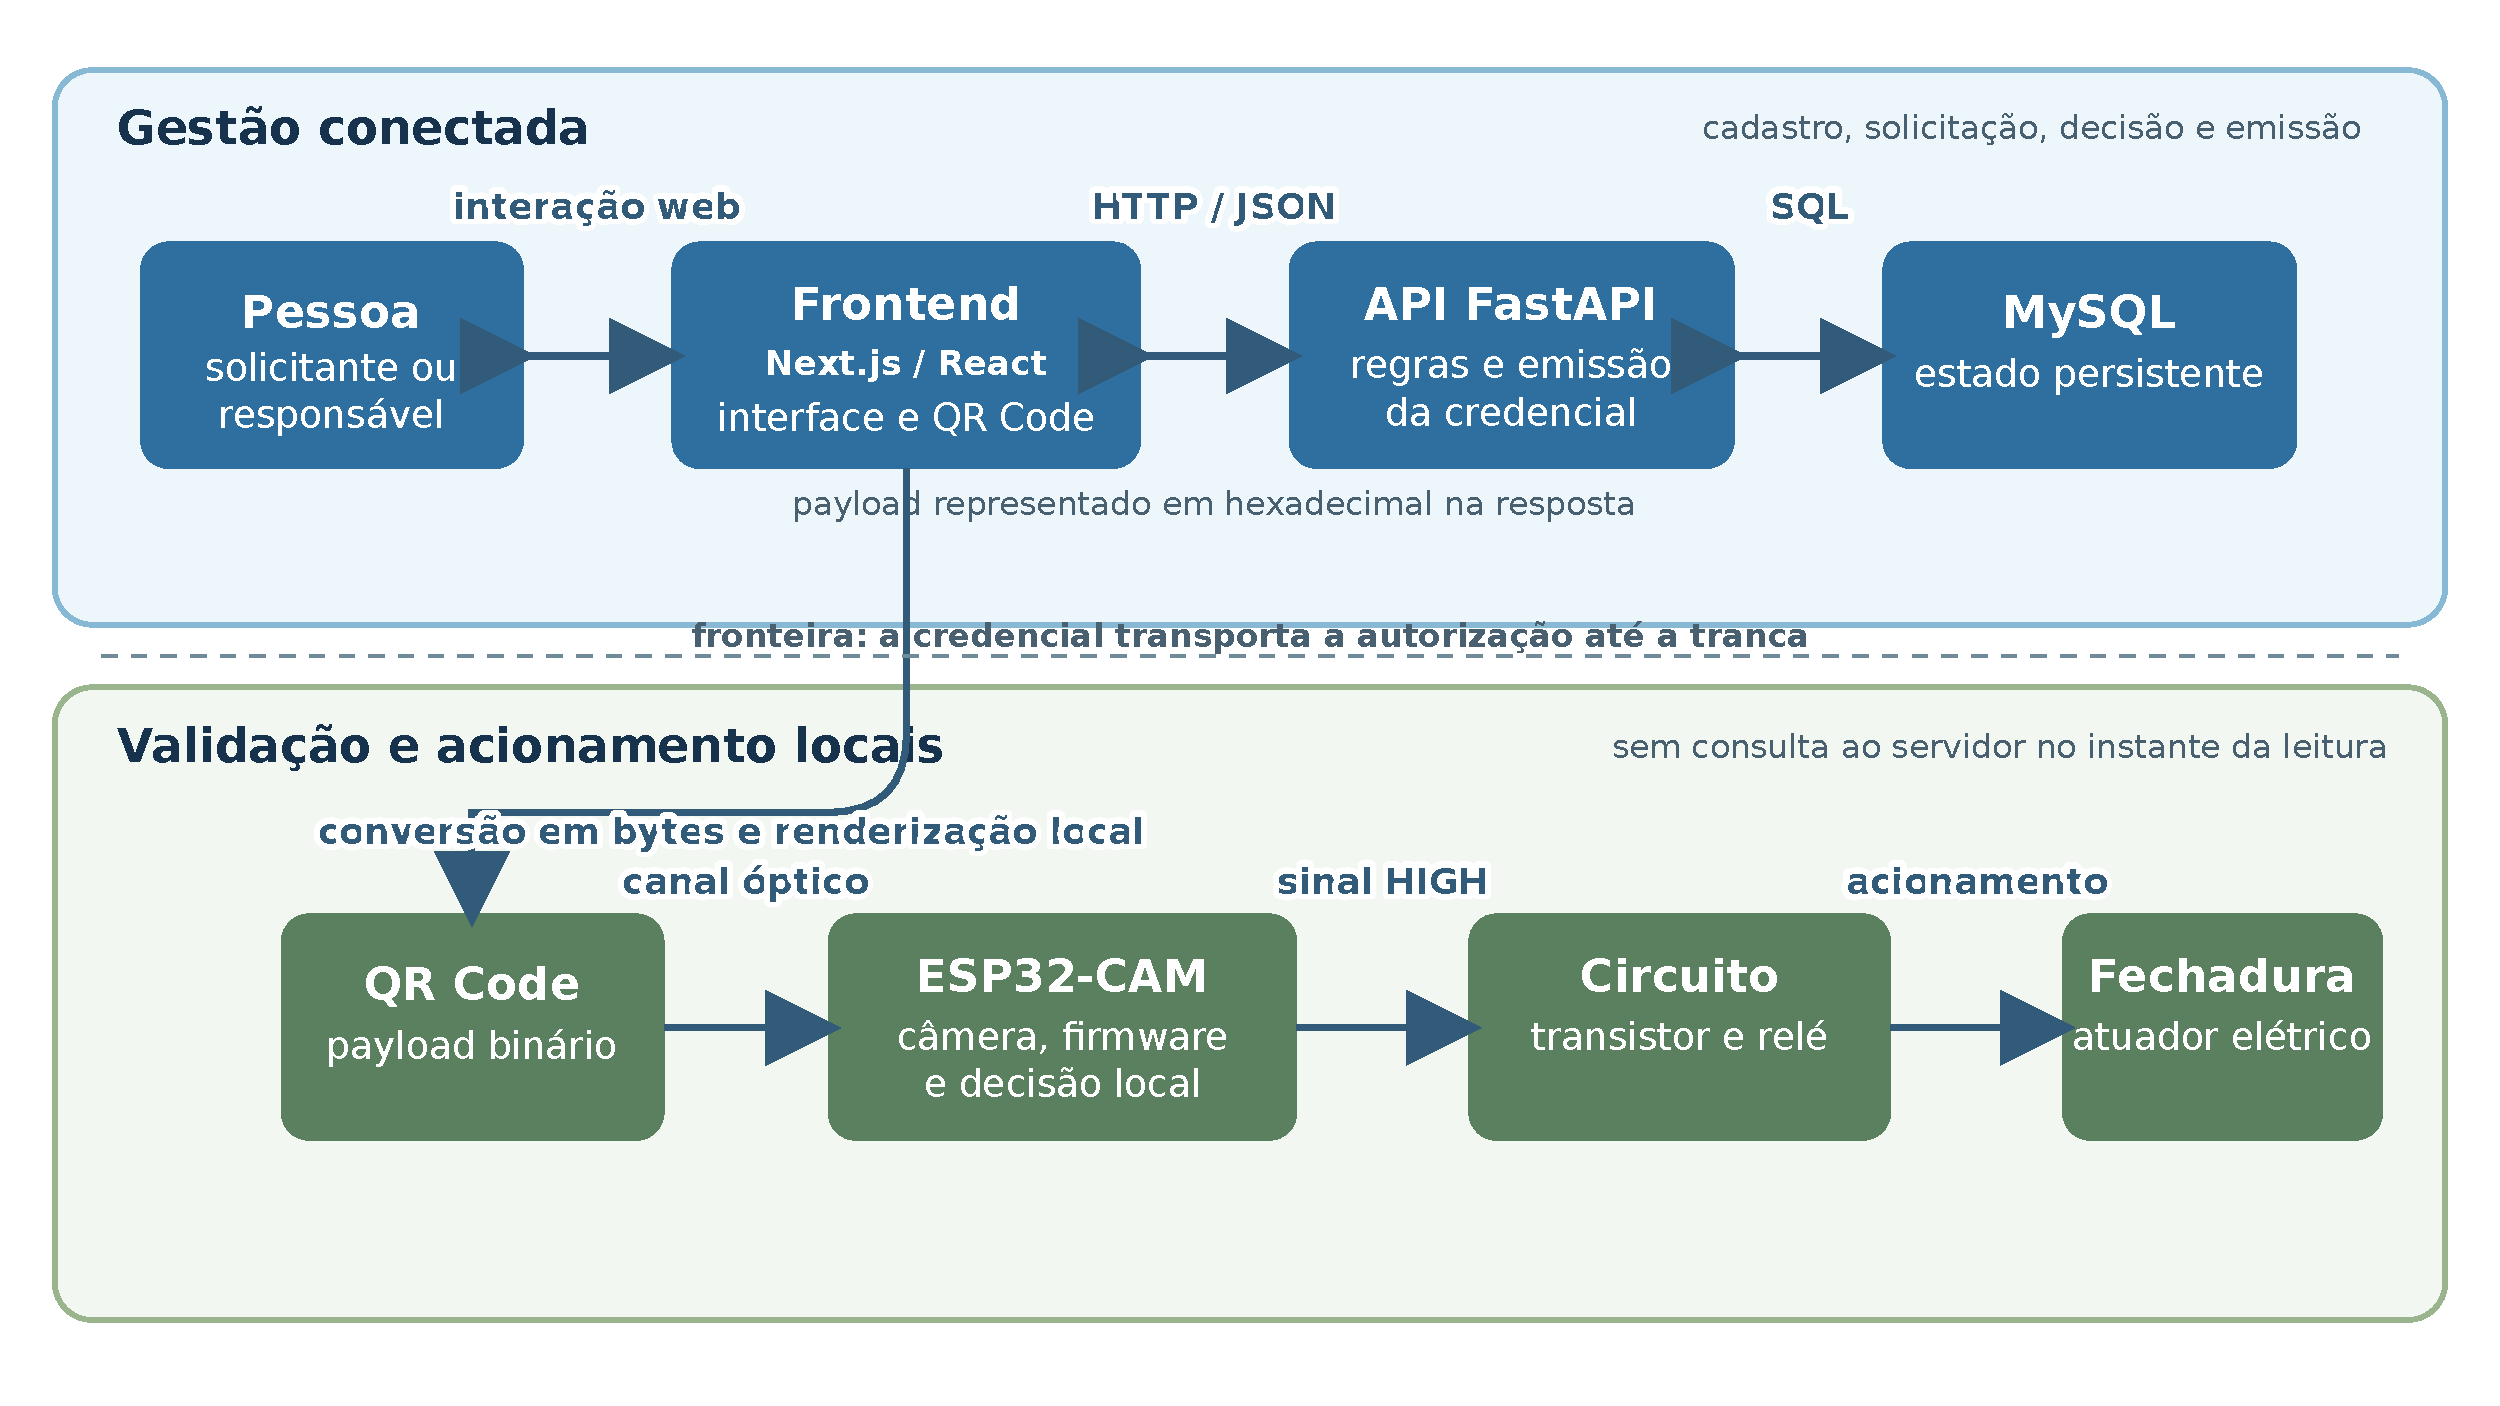
\includegraphics[width=\textwidth]{arquitetura_flike.pdf}
    \caption{Arquitetura geral e fronteira de operação do FLIKE}
    \label{fig:arquitetura-flike}
    \fonte{Elaborado pelos autores.}
\end{figure}

\subsection{Fronteira entre operação conectada e operação local}

Na região conectada da Figura~\ref{fig:arquitetura-flike}, o navegador, a API e o banco mantêm o estado administrativo. O usuário precisa acessar essa região para cadastrar-se, autenticar-se, solicitar uma credencial, acompanhar a decisão do responsável e recuperar o QR Code emitido. O FLIKE não implementa um aplicativo móvel nativo nem oferece gestão web independente do servidor.

A fronteira é atravessada pelo próprio payload apresentado visualmente. Depois que a credencial está disponível, a ESP32-CAM não precisa consultar o banco nem a API para decidir sobre a abertura: ela verifica localmente as informações autenticadas. Essa escolha evita que uma indisponibilidade momentânea da rede impeça a leitura de uma autorização já concedida, mas também impede que o dispositivo conheça imediatamente uma mudança realizada no servidor. As consequências para revogação, relógio e proteção do segredo serão discutidas na seção dedicada à operação local e à segurança.

A separação também delimita os registros produzidos em cada lado. Solicitação, aprovação e emissão pertencem ao estado central. Leitura, autorização e sinal de acionamento ocorrem no dispositivo. Sem um canal de sincronização e sem sensores adicionais, um registro no banco não equivale automaticamente à abertura da porta, e um comando elétrico não comprova entrada, saída ou ocupação.

\subsection{Decisões tecnológicas}

O frontend foi implementado com Next.js 16 e React 19, usando a organização de rotas pelo diretório \texttt{app}. O App Router do Next.js estrutura páginas e layouts por convenções do sistema de arquivos e integra os componentes React empregados pela interface \cite{vercel2026nextjs}. A escolha permitiu reunir no mesmo projeto as páginas de autenticação, solicitação, consulta e administração, além dos componentes e serviços que consomem a API.

O backend utiliza Python e FastAPI, com modelos Pydantic para representar entradas e saídas das rotas. A documentação oficial do framework destaca a integração entre anotações de tipo, validação de dados e geração de esquemas OpenAPI \cite{fastapi2026features}. No FLIKE, esses recursos organizam os contratos HTTP, enquanto as regras e o acesso ao banco permanecem distribuídos entre rotas, módulos e repositórios próprios do projeto.

A persistência foi implementada com MySQL e o conector oficial para Python. O modelo relacional permite expressar por chaves estrangeiras a hierarquia instituição--edifício--sala--tranca e os vínculos de usuários com solicitações e credenciais. A sintaxe e os tipos empregados seguem o sistema documentado no manual do MySQL \cite{oracle2026mysql84}; a estrutura concreta do FLIKE, entretanto, é definida pelos comandos de criação do próprio backend, apresentados na Subseção~\ref{subsec:modelo-dados}.

No dispositivo físico, a ESP32-CAM reúne câmera e capacidade de processamento para adquirir o QR Code e executar a validação próxima ao atuador. O QR Code foi adotado como transporte visual de dados binários, cuja capacidade depende da versão e do nível de correção de erros \cite{denso2012qressentials}. A autenticação do payload usa AES-CMAC, mecanismo simétrico que permite verificar a integridade e a origem criptográfica da mensagem sob a premissa de proteção do segredo compartilhado \cite{nist2005cmac}. O formato e as consequências de segurança dessas escolhas serão detalhados nas seções dedicadas à credencial digital e à operação local.

\section{Aplicação conectada e persistência}

A aplicação conectada reúne a interface, as regras de negócio e a persistência necessárias para transformar uma solicitação aprovada em credencial. Esta seção parte do modelo de domínio e de dados; as subseções posteriores descreverão a API, o frontend e o fluxo integrado de solicitação e emissão.

\subsection{Modelo de domínio e dados} \label{subsec:modelo-dados}

O esquema relacional foi reconstruído a partir dos comandos SQL de criação executados pelo backend. Essa fonte foi preferida ao arquivo DBML disponível no repositório porque o documento visual omite a tabela de solicitações e conserva uma versão anterior de campos da credencial. O diagrama da Figura~\ref{fig:modelo-dados-flike} representa, portanto, as nove tabelas efetivamente declaradas no script de inicialização e apenas as relações materializadas por chaves estrangeiras.

O núcleo institucional reúne relações sucessivas. \texttt{user} liga-se a \texttt{institution}; a hierarquia segue por \texttt{building} e \texttt{room} até chegar a \texttt{digital\_lock}. A coluna \texttt{owner\_id}, na tabela de instituições, associa cada instituição a um usuário e materializa a responsabilidade contextual: não existe tabela de administradores nem atributo global de papel. A mesma linha de \texttt{user} pode, assim, ser proprietária de instituições e também aparecer como solicitante ou titular de credenciais destinadas a trancas de outra instituição.

A tabela \texttt{digital\_key\_request} registra o usuário solicitante, a tranca destinatária e o estado \texttt{pending}, \texttt{approved} ou \texttt{rejected}. A tabela \texttt{digital\_key} armazena o usuário, a tranca, o payload de 48 bytes, a expiração e os campos de uso previstos pela aplicação. Ambas se ligam independentemente a \texttt{user} e \texttt{digital\_lock}: o esquema não possui uma chave estrangeira entre a solicitação aprovada e a credencial gerada. Essa ausência exige que a correspondência seja inferida pelo fluxo da aplicação e impede demonstrar somente pelo banco uma relação persistente e inequívoca entre os dois registros.

As credenciais de login ficam em \texttt{auth}, separadas dos dados de domínio em \texttt{user}. A associação entre as duas tabelas é conduzida pela aplicação a partir do e-mail transformado, mas não existe \texttt{user\_id} nem chave estrangeira que imponha essa correspondência no banco. Por esse motivo, a Figura~\ref{fig:modelo-dados-flike} usa uma linha tracejada para indicar a associação lógica e a distingue das relações referenciais declaradas pelo esquema.

Por fim, a tabela de eventos, \texttt{event\_log}, prevê registros associados a uma tranca. A tabela \texttt{digital\_key}, por sua vez, possui os campos \texttt{used} e \texttt{used\_at}. A existência dessas estruturas não demonstra coleta automática de eventos do dispositivo: o firmware não mantém comunicação com o backend durante a leitura. Esses campos representam possibilidades do modelo central e não devem ser interpretados como prova de abertura, passagem de uma pessoa ou ocupação do espaço.

\begin{figure}[p]
    \centering
    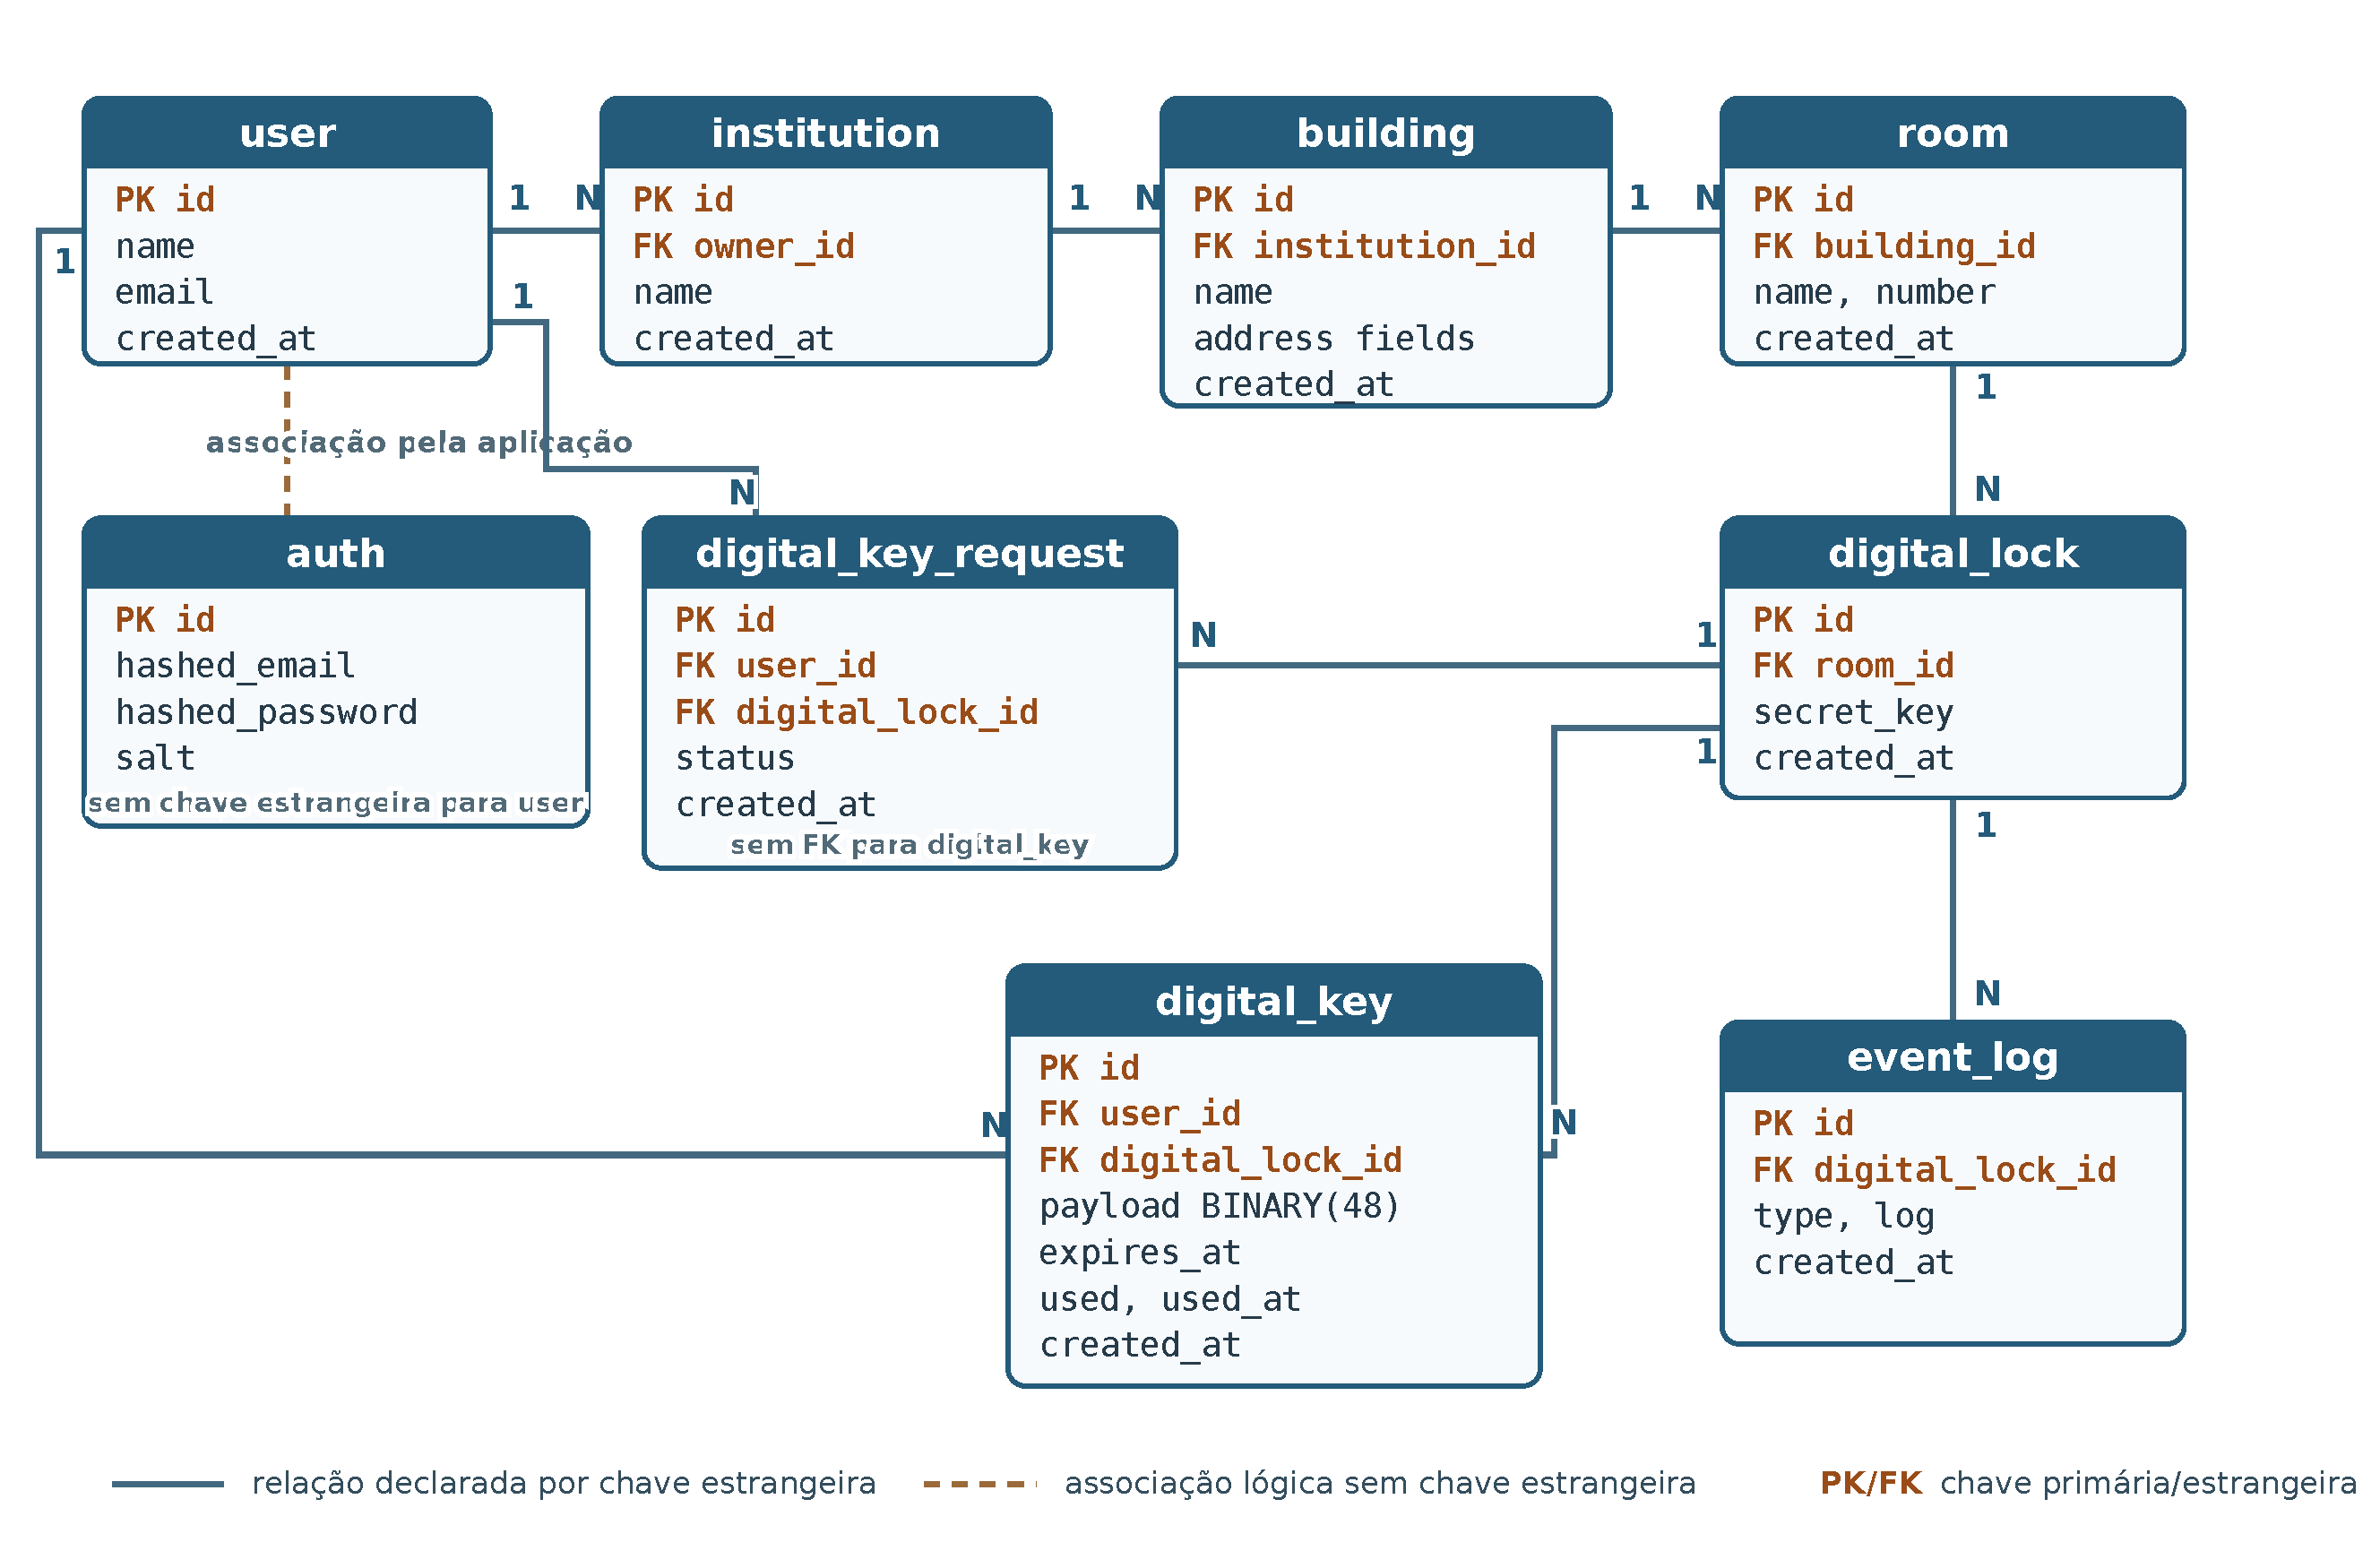
\includegraphics[width=\textwidth,height=0.76\textheight,keepaspectratio]{modelo_dados_flike.pdf}
    \caption{Modelo de dados efetivo do FLIKE}
    \label{fig:modelo-dados-flike}
    \fonte{Elaborado pelos autores a partir dos comandos SQL do backend.}
\end{figure}
\clearpage

\subsection{Backend}

A API organiza o código em rotas FastAPI, modelos Pydantic, repositórios e infraestrutura de persistência. As rotas recebem os parâmetros HTTP, selecionam o caso de uso e convertem exceções do domínio em respostas. Os modelos delimitam os corpos de entrada e parte das saídas. Os repositórios executam diretamente os comandos SQL de cada entidade, sem uma camada de mapeamento objeto--relacional, enquanto a infraestrutura fornece conexões MySQL obtidas de um pool. As regras de negócio ficam, portanto, distribuídas principalmente entre rotas e repositórios.

O cadastro cria os dados pessoais na tabela \texttt{user} e as credenciais na tabela \texttt{auth}. Nesta última, o e-mail é representado por seu hash e a senha recebe um salt aleatório antes da aplicação de SHA-256. No login, a API repete o cálculo e, se os valores coincidirem, emite um JSON Web Token (JWT). Esse formato transporta um conjunto de declarações entre partes de maneira compacta \cite{jones2015jwt}. Na implementação do FLIKE, o token é protegido com HS256, contém o identificador do usuário e a declaração de expiração, definida para uma hora após sua emissão. O segredo usado nesse mecanismo é uma configuração do servidor distinta do segredo AES-CMAC de cada tranca.

As rotas protegidas recebem o JWT no esquema Bearer, verificam sua integridade e validade e recuperam dele o identificador do usuário. A autorização administrativa não depende de uma classe global de administrador: para cada recurso, a API percorre tranca, sala, edifício e instituição até comparar \texttt{institution.owner\_id} com o usuário autenticado. Esse procedimento delimita consulta e manutenção de instituições, edifícios, salas e trancas próprias, assim como a decisão sobre solicitações destinadas a esses recursos.

As demais rotas podem ser agrupadas por sua função. O catálogo de acesso permite consultar a hierarquia institucional usada pelo solicitante. O conjunto de solicitações cria pedidos e os apresenta separadamente ao solicitante e ao responsável. As operações de decisão rejeitam o pedido ou emitem uma credencial. Por fim, as consultas de credenciais devolvem o payload em representação hexadecimal para que o frontend recupere seus bytes. Essa separação reflete dois contextos do mesmo usuário: solicitar acesso em instituições alheias e administrar a estrutura das instituições que possui.

Uma solicitação autenticada recebe o estado \texttt{pending}, a tranca informada e o identificador extraído do token. Antes de aprová-la ou rejeitá-la, a API confirma que ela permanece pendente e que sua tranca pertence ao responsável autenticado. A rejeição apenas altera o estado para \texttt{rejected}. Na aprovação, o backend cria uma credencial para o solicitante e a tranca e, em seguida, marca o pedido como \texttt{approved}. Quando a requisição não informa outra expiração, o padrão é 24 horas contadas do instante da aprovação e da emissão.

A política do projeto estabelece uma credencial para cada solicitação aprovada, mas essa cardinalidade não é imposta pelo esquema. Como visto na Subseção~\ref{subsec:modelo-dados}, não há chave estrangeira entre pedido e credencial. Além disso, a criação da credencial e a mudança do estado são confirmadas em operações separadas. O fluxo nominal produz a correspondência esperada, porém o banco, isoladamente, não permite reconstruí-la de modo inequívoco nem garante uma transição atômica diante de concorrência ou falha intermediária.

A cobertura de autenticação do commit examinado é parcial. As rotas sob o prefixo administrativo e as operações referentes ao próprio perfil e às próprias solicitações exigem JWT. Em contrapartida, listagens gerais de usuários e da estrutura institucional, consultas de credenciais e operações diretas sobre credenciais não aplicam a mesma dependência. As consultas públicas por usuário ou por identificador devolvem o payload, e as respostas das rotas públicas de trancas incluem \texttt{secret\_key} em hexadecimal.

Essa última exposição rompe uma premissa central do modelo de segurança: quem obtiver o segredo de uma tranca poderá produzir tags AES-CMAC válidas para ela. Assim, a implementação examinada não sustenta uma alegação de proteção efetiva do segredo, ainda que a arquitetura pressuponha seu armazenamento restrito ao backend e ao dispositivo. O fechamento dessas rotas e a exclusão do segredo das respostas são correções necessárias antes de qualquer implantação. As consequências para o modelo de ameaça serão retomadas na seção dedicada à segurança.

\subsection{Frontend}

O frontend utiliza as rotas do App Router para compor as páginas visíveis. Componentes reutilizáveis implementam tabelas, cartões, formulários e modais; hooks coordenam estado, carregamento, mensagens de erro e ações; serviços concentram as requisições HTTP; e tipos TypeScript representam os dados trocados com a API. Essa divisão permite que uma página reúna a apresentação e delegue a comunicação e as transições de estado às demais unidades.

Após o cadastro, o usuário autentica-se e o JWT é guardado pelo navegador. A implementação usa o armazenamento local, denominado \textit{localStorage} pela API Web, sob a chave \texttt{access\_token}. As páginas conectadas verificam sua presença para redirecionar ao login, mas essa verificação local não valida o token nem constitui autorização. A decisão efetiva ocorre quando uma rota protegida da API valida o Bearer recebido. Não há, no código examinado, middleware global de sessão, renovação do token ou persistência do login fora do armazenamento do navegador.

No fluxo de solicitação, a interface conduz o usuário pela seleção sucessiva de instituição, edifício e sala. Depois da escolha da sala, o hook consulta as trancas associadas e utiliza a primeira retornada pela API; a versão examinada não apresenta ao usuário uma escolha quando há múltiplas trancas. A ação final envia apenas o identificador dessa tranca, pois o backend deriva do JWT a identidade do solicitante. Uma confirmação textual informa que o pedido foi registrado.

O painel do solicitante combina os dados do usuário, suas credenciais e os pedidos rejeitados. Para apresentar uma credencial, o frontend consulta o registro pelo identificador, separa os pares hexadecimais, reconstrói um vetor de bytes e o entrega à biblioteca de QR Code em modo binário. O resultado é uma URL de dados exibida em um modal. Essa geração ocorre no navegador e não cria nova credencial no servidor. Também não implementa, por si só, download dedicado, funcionamento como aplicativo móvel ou persistência da imagem depois de uma recarga.

A classificação exibida no painel ainda considera ativa apenas a credencial não marcada como usada e cuja expiração está no futuro. Esse critério conserva a semântica legada do campo \texttt{used}, mas não representa a política final do FLIKE: a mesma credencial pode ser reapresentada durante sua janela de validade. Por isso, a marcação de uso da aplicação conectada não será empregada como regra de autorização física.

No fluxo do responsável, a mesma aplicação apresenta somente instituições, edifícios, salas e trancas que pertencem ao usuário autenticado. A tela de pedidos permite filtrar os estados \texttt{pending}, \texttt{approved} e \texttt{rejected}. Os botões de aprovação e rejeição aparecem para pedidos pendentes e, depois da resposta da API, a listagem é consultada novamente. Embora os caminhos e rótulos da interface usem o termo administrativo, a permissão continua derivada da propriedade da instituição.

\subsection{Fluxo de solicitação e emissão}

A Figura~\ref{fig:fluxo-solicitacao-emissao} reúne o caminho principal sem antecipar o formato interno da credencial. Na primeira etapa, o solicitante escolhe a tranca por meio da aplicação. O frontend envia o pedido autenticado, a API associa o usuário extraído do token e o banco persiste o estado pendente. A resposta confirma o registro, mas ainda não contém uma autorização.

Na segunda etapa, o responsável consulta os pedidos relacionados às instituições que possui. Quando envia sua decisão, a API verifica novamente a propriedade da tranca e o estado do pedido. Uma rejeição encerra o fluxo administrativo sem credencial. Uma aprovação cria o payload autenticado, persiste a credencial e altera o pedido para \texttt{approved}. Por padrão, sua janela termina 24 horas depois desse instante; uma expiração diferente pode ser informada no contrato da API.

\begin{figure}[htbp]
    \centering
    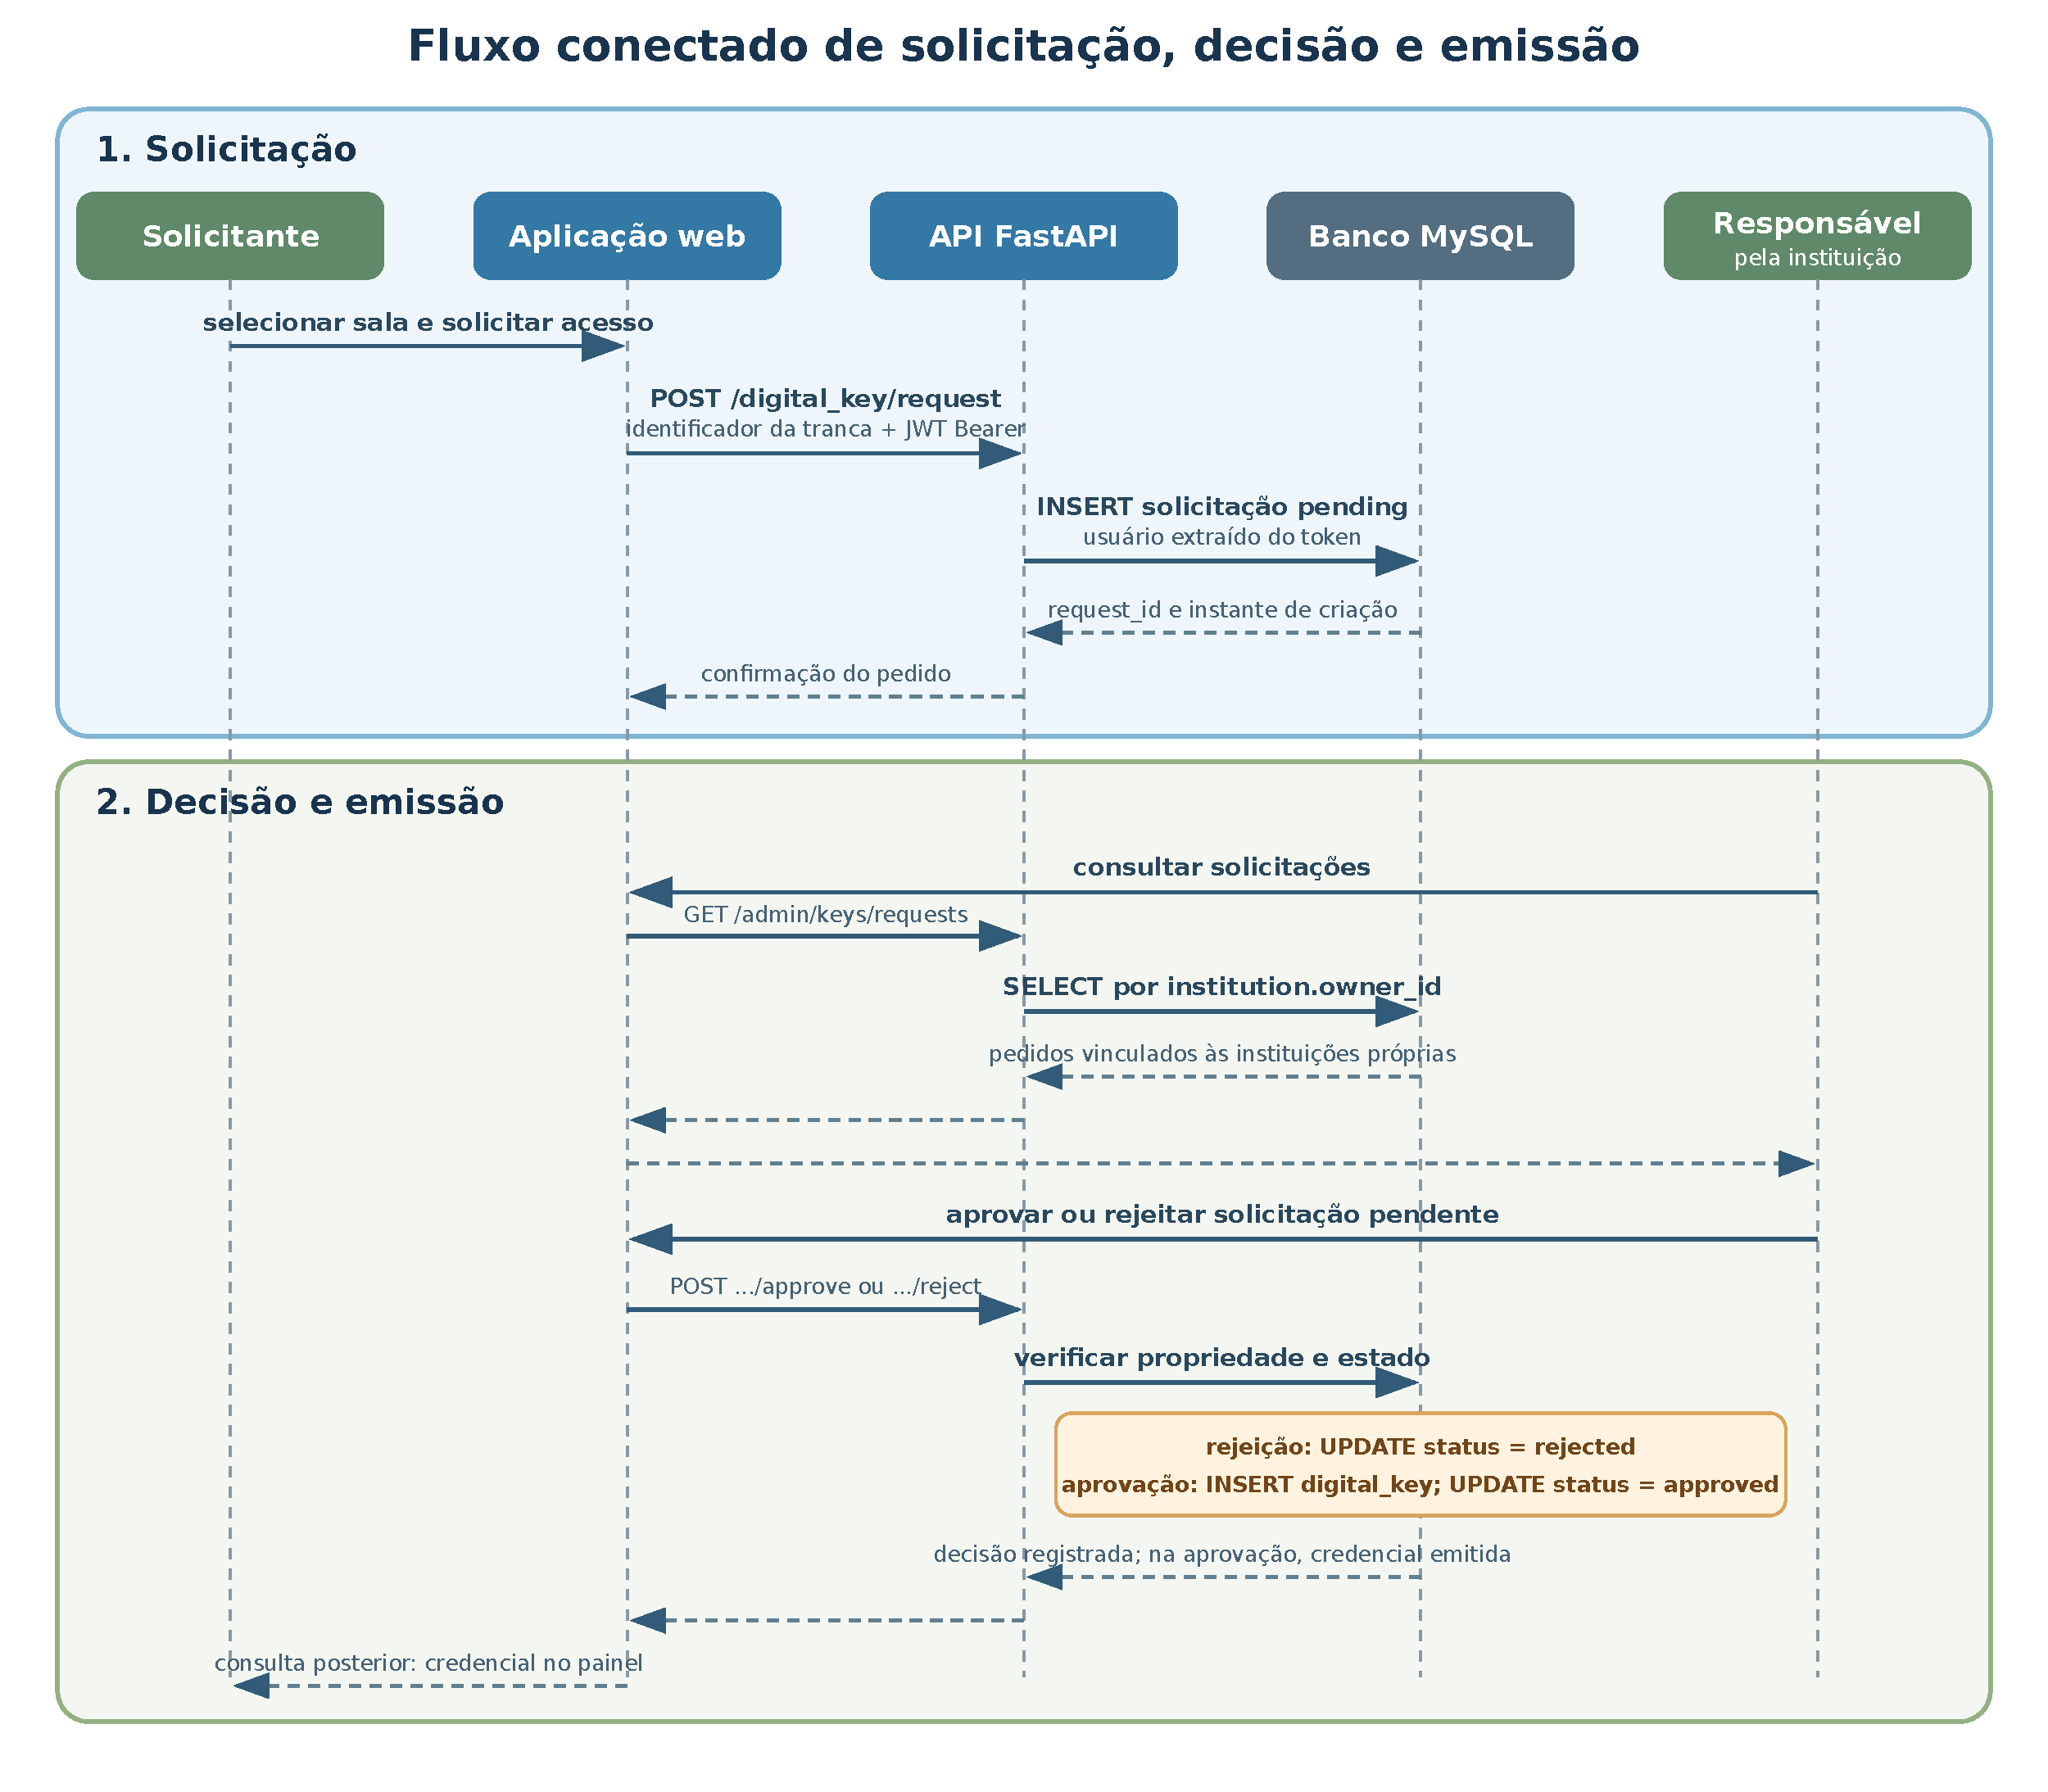
\includegraphics[width=\textwidth,height=0.78\textheight,keepaspectratio]{fluxo_solicitacao_emissao.pdf}
    \caption{Sequência de solicitação, decisão e emissão da credencial}
    \label{fig:fluxo-solicitacao-emissao}
    \fonte{Elaborado pelos autores a partir da implementação do FLIKE.}
\end{figure}

Em consulta posterior, o painel do solicitante recupera a credencial emitida e renderiza o QR Code. A obtenção do payload depende da aplicação conectada; somente a leitura e a decisão junto à fechadura dispensam consulta ao servidor. A aprovação, a emissão, a obtenção da imagem e a apresentação física são eventos distintos. Uma única emissão nominal decorre da solicitação aprovada, enquanto a credencial resultante permanece reapresentável até o instante de expiração, exclusive.

\section{Credencial digital}

\subsection{Conceito e ciclo de vida}

A credencial digital é a representação portável de uma autorização temporária. Ela nasce quando o responsável aprova uma solicitação, permanece associada ao usuário lógico e a uma tranca específica e deixa de ser aceita ao término do intervalo concedido. Solicitação, credencial e QR Code têm papéis distintos: a solicitação registra o pedido e sua decisão; a credencial reúne os dados autenticados da autorização; e o QR Code é somente o meio óptico pelo qual os bytes chegam ao dispositivo.

O segredo criptográfico também não integra a credencial. O backend e a tranca destinatária possuem previamente uma cópia desse valor, provisionado no dispositivo pelo fornecedor na programação da ESP32-CAM. O servidor usa o segredo para produzir o código de autenticação, e o dispositivo o usa para verificar o código recebido. Esse arranjo permite a decisão local, mas faz da proteção do segredo uma premissa de segurança do sistema.

O ciclo nominal possui quatro transições. Primeiro, o servidor registra a solicitação pendente. Segundo, o responsável a aprova ou rejeita. Terceiro, somente uma aprovação produz a credencial, cuja emissão inicia a janela de autorização. Quarto, o titular apresenta o QR Code à tranca durante essa janela. A apresentação não consome a autorização: o mesmo símbolo pode ser lido novamente até o instante de expiração.

\subsection{Informações autenticadas}

O conteúdo protegido reúne quatro valores. \texttt{user\_id} identifica a conta à qual a autorização foi concedida; \texttt{digital\_lock\_id} identifica a tranca lógica destinatária; \texttt{issued\_at} registra o primeiro instante admissível; e \texttt{expires\_at} marca o limite superior, que já não pertence ao intervalo. O usuário físico não é autenticado pela apresentação: quem obtiver uma cópia do QR Code poderá reapresentá-lo enquanto ele for válido.

Os instantes são representados como segundos inteiros desde a época POSIX. A condição temporal adotada é

\begin{equation}
    \texttt{issued\_at} \leq \texttt{agora} < \texttt{expires\_at}.
\end{equation}

Essa definição evita ambiguidade na fronteira: a credencial vale no instante de emissão, inclusive, e deixa de valer no instante de expiração, exclusive. A comparação depende de um relógio coerente no dispositivo; operar sem servidor não elimina essa dependência temporal.

\subsection{Serialização e autenticação}

Antes do cálculo criptográfico, cada um dos quatro valores é convertido em um inteiro sem sinal de 64 bits, em ordem de bytes do mais significativo para o menos significativo (\textit{big-endian}). A concatenação produz 32 bytes de dados. Sobre essa sequência, o backend calcula uma tag AES-CMAC de 16 bytes com uma chave AES de 256 bits e a anexa ao final. O payload completo possui, como consequência, 48 bytes. O Quadro~\ref{qua:layout-credencial} apresenta o leiaute.

\begin{quadro}[htb]
    \caption{Leiaute binário da credencial do FLIKE}
    \label{qua:layout-credencial}
    \small
    \setlength{\tabcolsep}{4pt}
    \begin{tabular}{|p{0.20\textwidth}|p{0.12\textwidth}|p{0.18\textwidth}|p{0.40\textwidth}|}
        \hline
        \textbf{Campo} & \textbf{Bytes} & \textbf{Intervalo} & \textbf{Função} \\ \hline
        \texttt{user\_id} & 8 & 0--7 & Identificar a conta autorizada. \\ \hline
        \texttt{digital\_lock\_id} & 8 & 8--15 & Vincular a autorização à tranca destinatária. \\ \hline
        \texttt{issued\_at} & 8 & 16--23 & Delimitar o início da autorização em tempo POSIX. \\ \hline
        \texttt{expires\_at} & 8 & 24--31 & Delimitar o fim exclusivo da autorização. \\ \hline
        tag AES-CMAC & 16 & 32--47 & Autenticar conjuntamente os 32 bytes anteriores. \\ \hline
    \end{tabular}
    \fonte{Elaborado pelos autores a partir da implementação do backend.}
\end{quadro}

O CMAC é um código de autenticação de mensagem baseado em cifra de bloco. Sob a premissa de que somente os componentes autorizados conhecem a chave, a coincidência da tag fornece evidência de que os dados foram produzidos por alguém que possui esse segredo e não foram alterados sem a recomputação do código \cite{nist2005cmac}. O mecanismo não oculta os identificadores nem os instantes, não impede a cópia de uma mensagem autêntica e não produz assinatura digital ou não repúdio. A comparação deve abranger a tag completa, e qualquer diferença deve resultar em rejeição.

\subsection{Codificação em QR Code}

O frontend recebe o payload em hexadecimal, converte cada par para o byte correspondente e entrega o vetor à biblioteca de QR Code em modo binário. Essa etapa é necessária porque tratar o conteúdo como texto introduziria uma nova codificação e poderia alterar bytes nulos ou valores superiores a \texttt{0x7f}. O símbolo final é fixado na versão 3, cuja matriz possui 29 por 29 módulos, e usa nível L de correção de erros.

A escolha decorreu de um limite observado durante o desenvolvimento: símbolos mais densos eram lidos com menor facilidade pela câmera do protótipo. O formato binário compacto possibilitou transportar os 48 bytes na versão 3-L, mantendo a matriz menor. O nível L reserva menos redundância do que níveis superiores e, portanto, aceita menor dano físico; trata-se de um compromisso entre capacidade, densidade óptica e tolerância a degradação, não de uma propriedade criptográfica \cite{denso2012qressentials}. Além disso, o QR Code não é um canal confiável por natureza: ele pode ser copiado ou substituído, razão pela qual a decisão depende do conteúdo autenticado e do destino conferido pelo firmware \cite{kieseberg2010qrcode}.

\subsection{Decisão de aceitação}

A leitura bem-sucedida inicia a validação, mas não autoriza o acesso. O dispositivo confirma o comprimento completo, separa dados e tag, recalcula o AES-CMAC, compara o identificador destinatário e avalia a janela temporal. Somente a conjunção dessas condições produz o sinal lógico de abertura. A Figura~\ref{fig:validacao-local-flike} representa o fluxo; sua ordem gráfica não altera a exigência de que todas as verificações precedam o acionamento.

\begin{figure}[htbp]
    \centering
    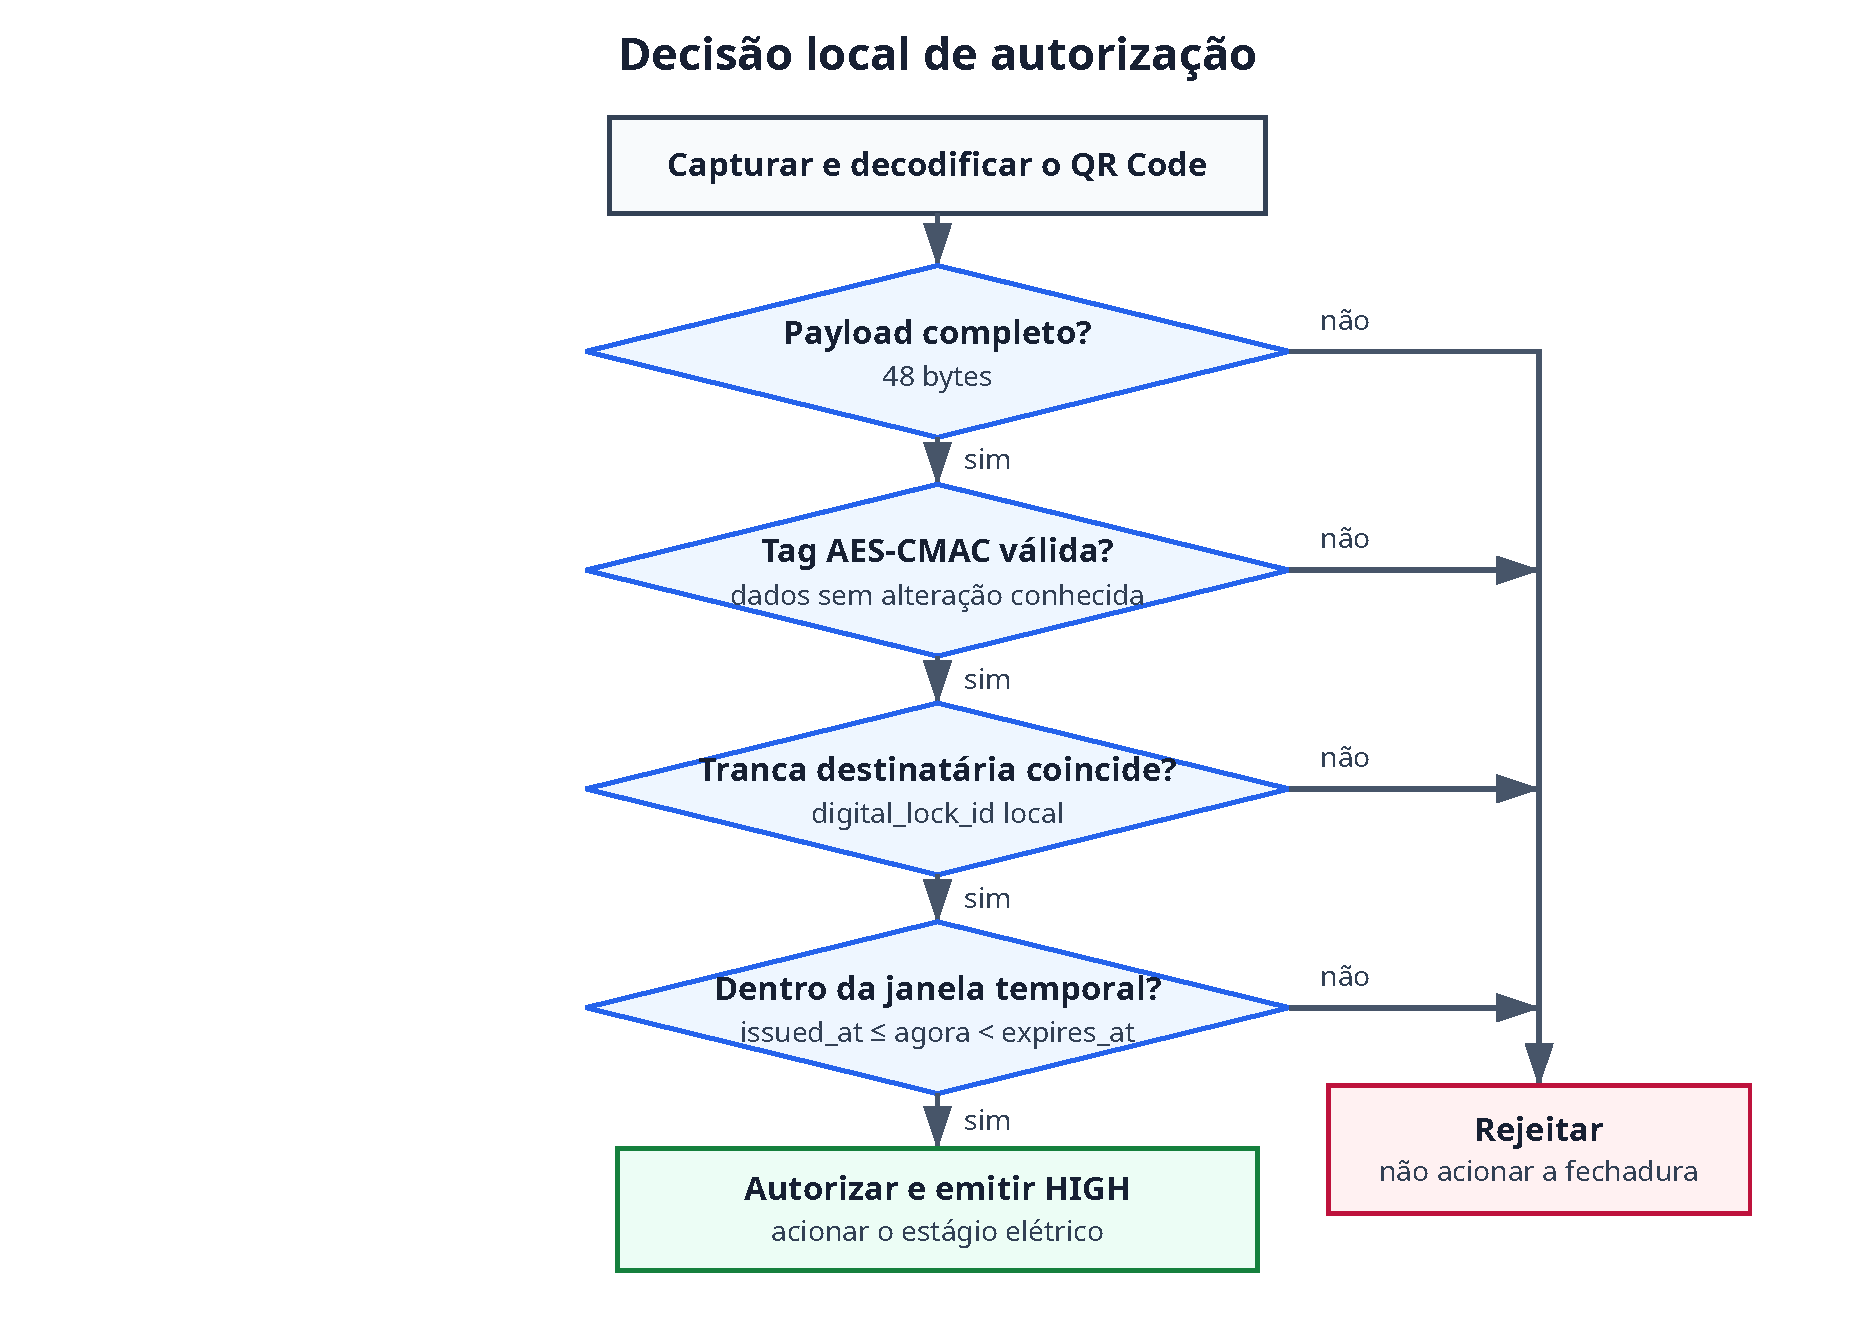
\includegraphics[width=0.90\textwidth,height=0.78\textheight,keepaspectratio]{validacao_local_flike.pdf}
    \caption{Fluxo local de validação da credencial}
    \label{fig:validacao-local-flike}
    \fonte{Elaborado pelos autores.}
\end{figure}

Uma tag válida para outra tranca continua sendo uma mensagem autêntica, mas não uma autorização para o atuador que a recebeu. De forma semelhante, uma mensagem autêntica e destinada ao dispositivo ainda deve ser recusada fora do intervalo temporal. O estado \texttt{used} mantido no banco não participa dessa decisão, pois o dispositivo deliberadamente não consulta o servidor e a política final permite reapresentações durante a vigência.

\section{Dispositivo físico}

\subsection{Plataforma embarcada e aquisição do QR Code}

O dispositivo foi construído com uma placa ESP32-CAM no arranjo AI-Thinker e uma câmera OV2640. A biblioteca de leitura inicializa a câmera, executa a aquisição em uma tarefa do sistema operacional de tempo real e disponibiliza o vetor bruto e seu comprimento ao laço principal. O processamento preserva o tamanho fornecido pelo decodificador; ele não interpreta a credencial como cadeia de caracteres terminada por zero.

A ESP32 integra processador, memória, periféricos digitais e recursos de comunicação adequados à prototipação de sistemas embarcados. No FLIKE, sua função relevante é concentrar aquisição óptica, validação da credencial e geração do sinal de controle próximo ao atuador. O produto não depende de seus rádios durante a decisão de acesso. A ausência de tráfego nesse instante reduz a dependência operacional, mas não transforma a placa em componente endurecido contra extração física de segredo.

\subsection{Firmware de validação}

O firmware preservado no repositório registra a integração entre a biblioteca da câmera e o cálculo AES-CMAC da biblioteca Mbed TLS. Ele separa os 32 bytes de dados dos 16 bytes finais, recalcula a tag com AES-256 e compara o resultado. Essa versão arquivada imprime o conteúdo e o resultado no monitor serial; não contém, no mesmo commit, todas as verificações e o acionamento usados no ensaio final.

Na versão gravada para a demonstração integrada, o processamento também confirmou o comprimento, recuperou os quatro inteiros em ordem \textit{big-endian}, comparou \texttt{digital\_lock\_id} com o identificador provisionado, avaliou \texttt{issued\_at} e \texttt{expires\_at} e emitiu \texttt{HIGH} somente após a aceitação. O código-fonte exato desse ensaio não foi preservado no repositório. Essa lacuna impede reproduzir a imagem de firmware a partir do controle de versão, mas não elimina o resultado observado na demonstração física, descrito na Subseção~\ref{subsec:demonstracao-fisica}.

\subsection{Circuito de acionamento}

O estágio elétrico reaproveita a topologia construída pelos autores em um projeto anterior da disciplina Laboratório de Processadores, antecedente histórico do FLIKE. O sinal lógico da ESP32-CAM chega à base de um transistor NPN 2N2222 por um resistor de 1~k$\Omega$. O transistor funciona como chave e condiciona o comando aplicado à entrada do módulo de relé de 12~V; um segundo resistor de 1~k$\Omega$ estabelece o nível de repouso. O contato normalmente aberto do relé comuta a alimentação da fechadura Papaiz AA-ERL200P.

O circuito usa duas alimentações. Um carregador de celular adaptado fornece a baixa tensão da ESP32-CAM, enquanto uma fonte chaveada de 12~V alimenta relé e fechadura. Essa separação permite que o pino digital controle uma carga que não pode ser acionada diretamente pelo microcontrolador. A Figura~\ref{fig:circuito-eletrico-flike} registra a topologia; o ramo de acionamento manual representado no esquema foi previsto, mas não montado no protótipo avaliado.

\begin{figure}[p]
    \centering
    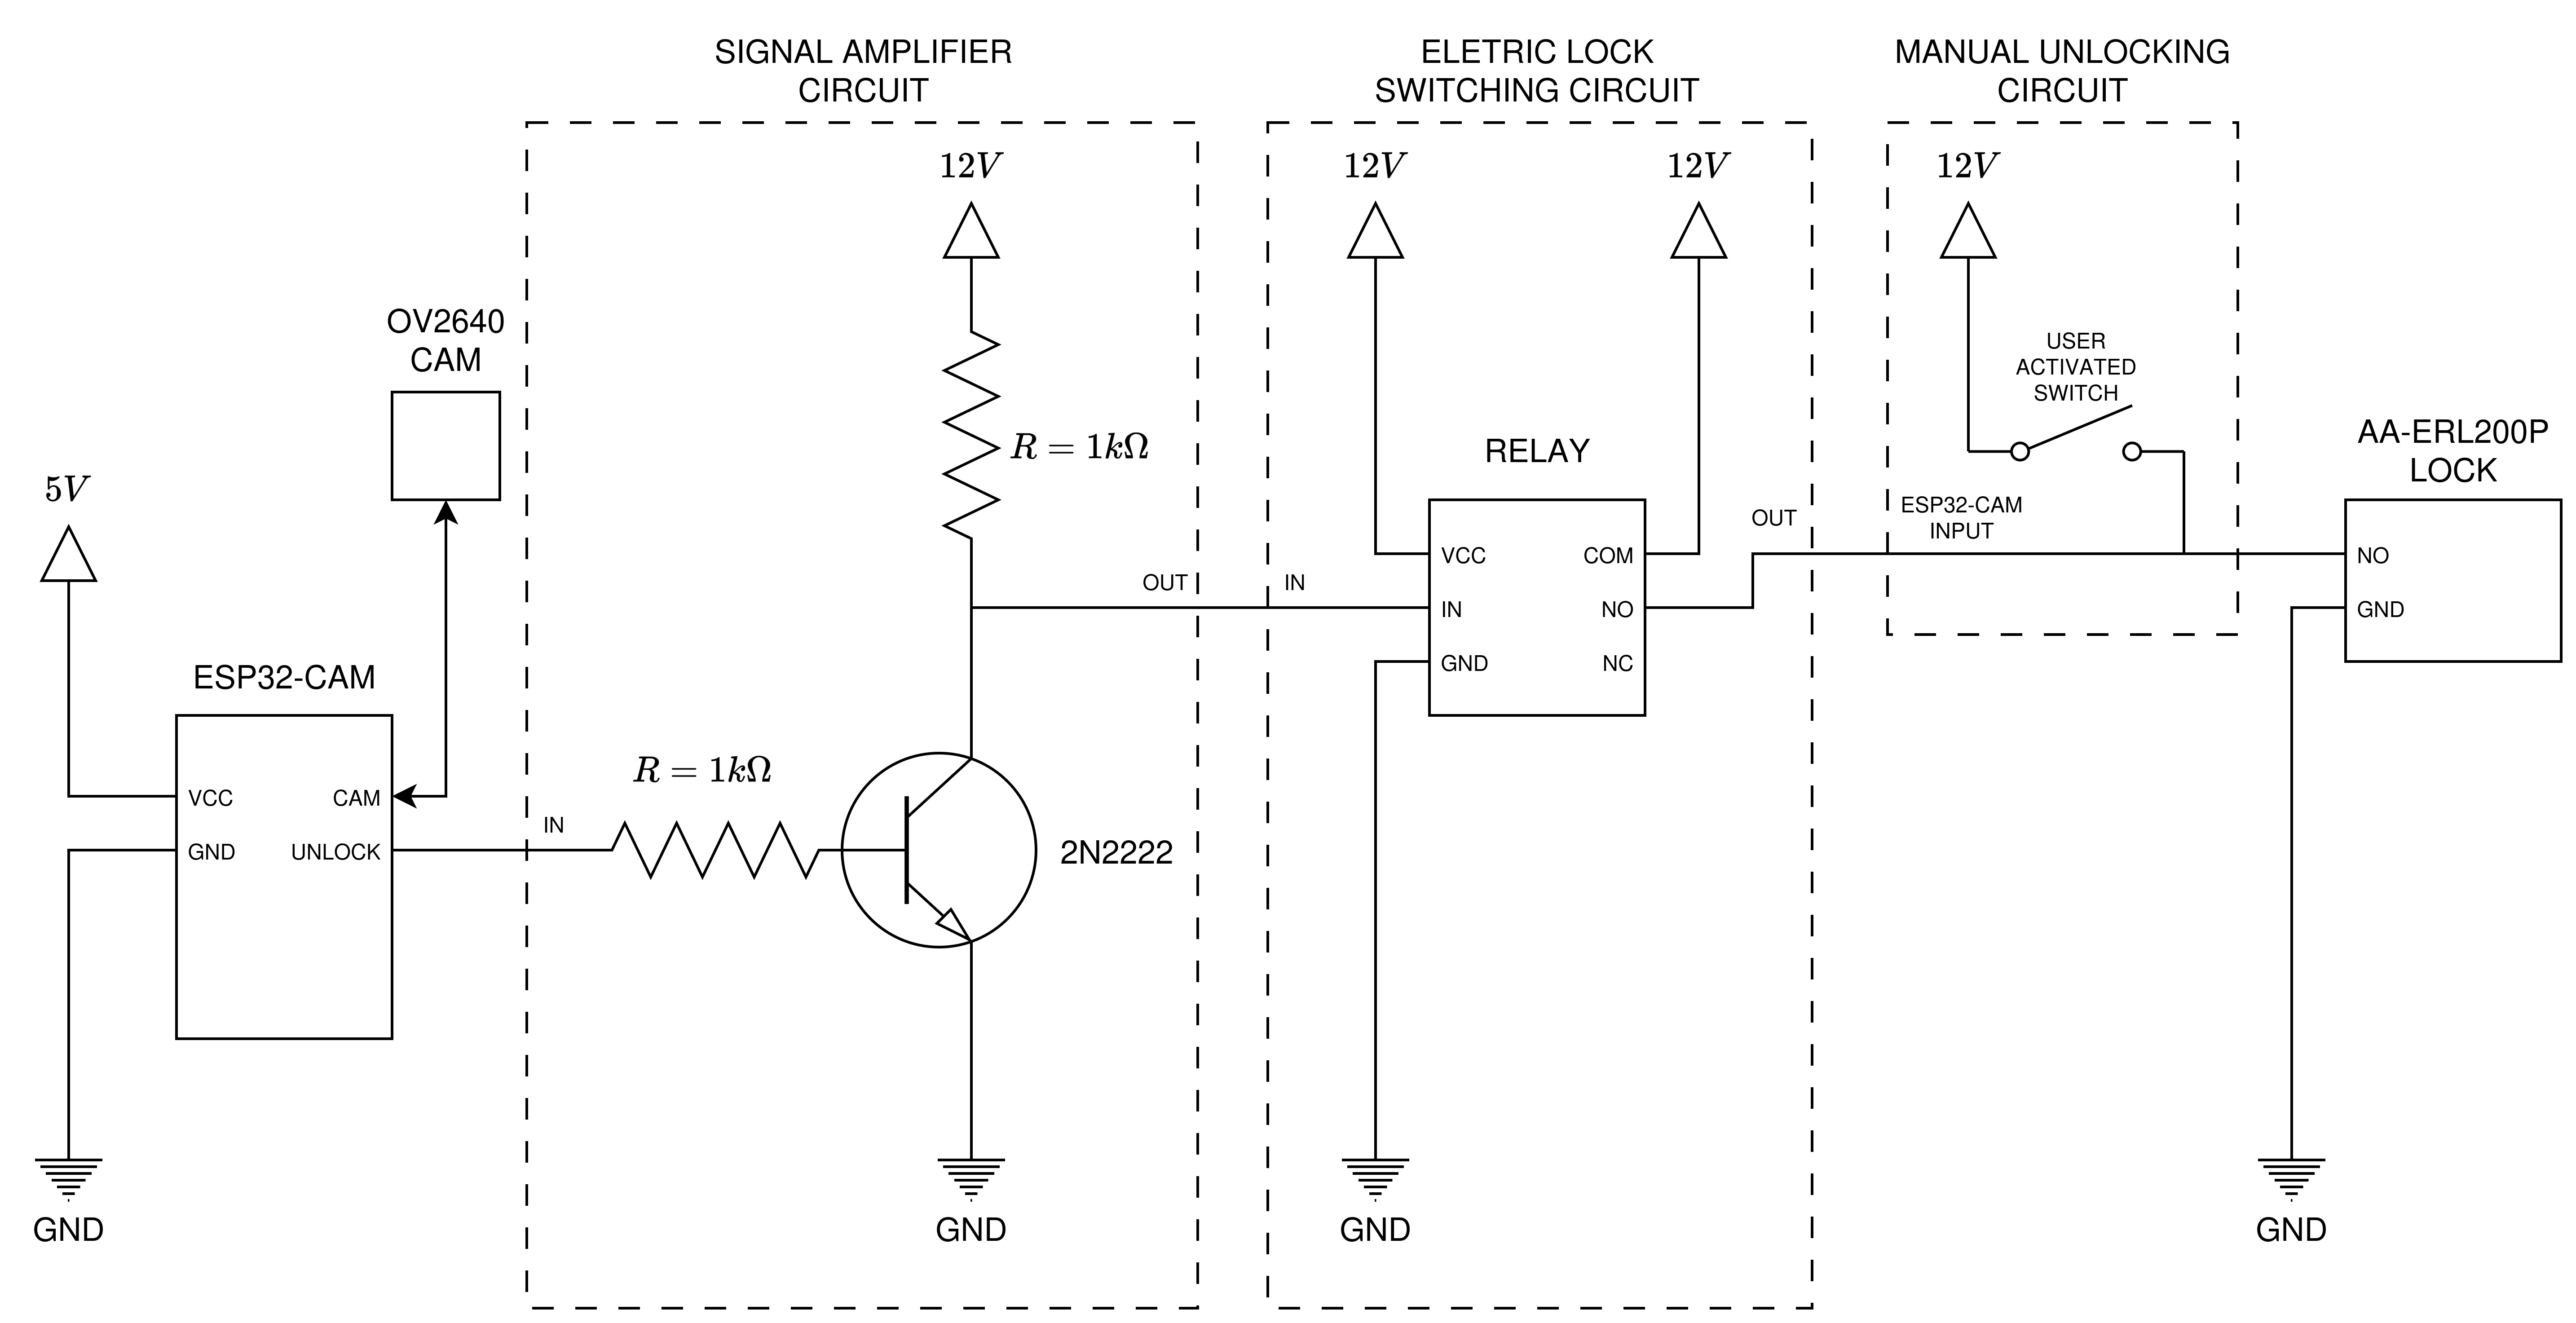
\includegraphics[width=\textwidth,height=0.78\textheight,keepaspectratio]{circuito_eletrico_flike.png}
    \caption{Esquema elétrico do estágio de acionamento empregado no FLIKE}
    \label{fig:circuito-eletrico-flike}
    \fonte{Elaborado pelos autores.}
\end{figure}
\clearpage

O protótipo é uma montagem de bancada em protoboard, sem placa dedicada, gabinete, bateria ou certificação elétrica. O relé oferece separação funcional entre comando e carga, mas o projeto não avaliou isolação, imunidade eletromagnética, aquecimento, durabilidade ou adequação a uma instalação permanente. A Figura~\ref{fig:prototipo-flike} identifica os componentes principais da montagem.

\begin{figure}[htbp]
    \centering
    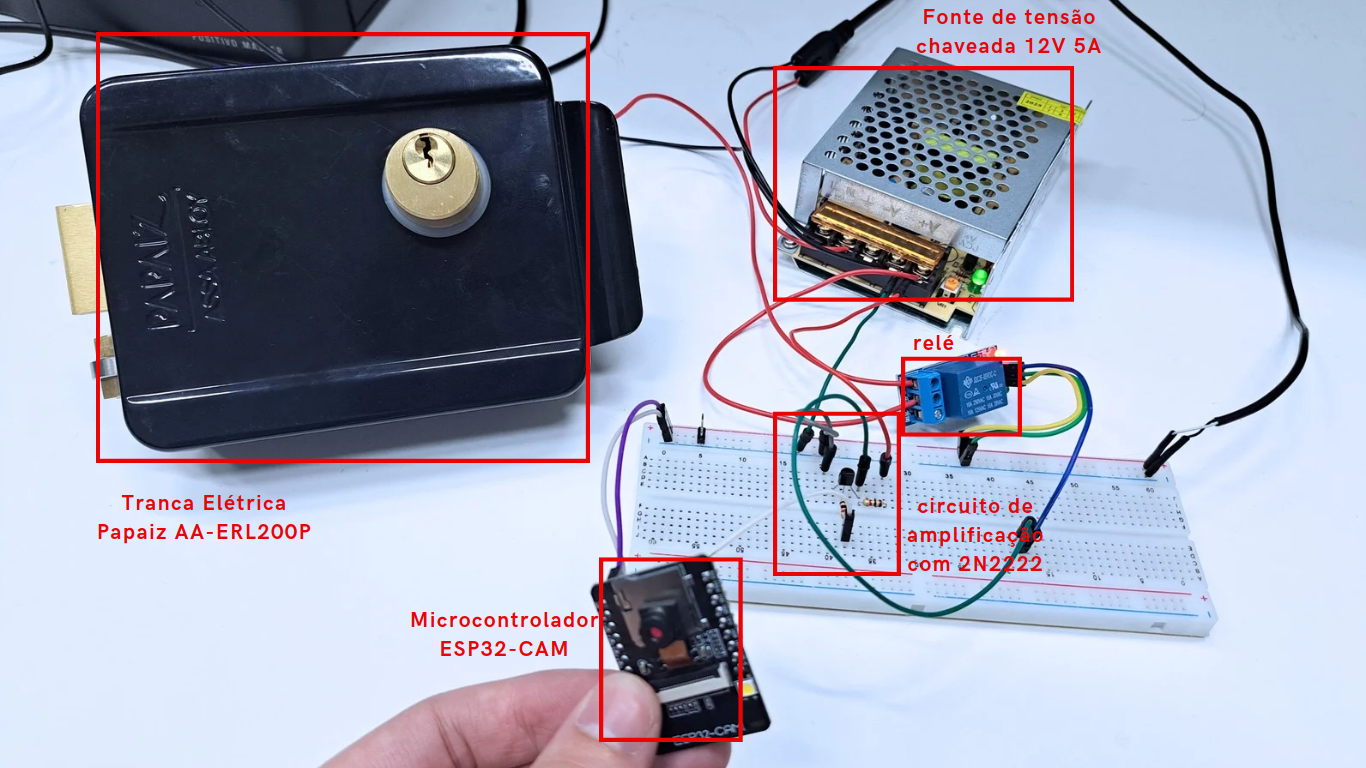
\includegraphics[width=\textwidth,height=0.72\textheight,keepaspectratio]{prototipo_flike_anotado.png}
    \caption{Protótipo experimental do circuito de acionamento}
    \label{fig:prototipo-flike}
    \fonte{Acervo dos autores.}
\end{figure}

\subsection{Demonstração física} \label{subsec:demonstracao-fisica}

A equipe realizou uma demonstração física ponta a ponta do FLIKE em 31 de agosto de 2026. Uma credencial foi apresentada à câmera; o dispositivo reconheceu o QR Code, recuperou os 48 bytes, extraiu os campos e verificou comprimento, tranca destinatária, instante de emissão, expiração e tag AES-CMAC. Diante do caso válido, o microcontrolador emitiu o nível \texttt{HIGH}; o transistor comandou o relé; e a fechadura elétrica foi acionada.

O ensaio estabeleceu a continuidade funcional entre canal óptico, decisão embarcada e carga elétrica. Seu registro disponível é o relato concordante da equipe, apoiado pelo código preservado dos subsistemas, pelo esquema e pela fotografia da montagem. Não foram preservados vídeo, log serial ou imagem binária do firmware do ensaio. Consequentemente, o resultado sustenta que a integração ocorreu, mas não permite calcular taxa de sucesso, tempo médio de leitura, tolerância a ângulo ou iluminação, consumo, repetibilidade estatística ou confiabilidade de longo prazo.

O evento observado foi o acionamento da fechadura. Como não há sensor de estado da porta, de passagem ou de ocupação, o sistema não distingue automaticamente destravamento, abertura física, entrada, saída e permanência no ambiente.

\section{Operação local, segurança e auditoria}

\subsection{Consequências da operação sem servidor}

A decisão local permite utilizar uma credencial já emitida quando o dispositivo não possui acesso à API. Essa propriedade cobre leitura, validação e acionamento; cadastro, solicitação, aprovação, emissão e recuperação inicial do QR Code continuam conectados. Ela exige que identificador, segredo e relógio estejam disponíveis localmente.

O mesmo isolamento impede revogação imediata. Depois da emissão, retirar a permissão no banco não informa a tranca sem um canal adicional; a credencial poderá ser aceita até \texttt{expires\_at}. Janelas curtas reduzem a duração desse risco, mas aumentam a frequência de emissão e a dependência do serviço web. O padrão de 24 horas adotado no backend é uma política do protótipo e deve ser ajustado ao risco do espaço em uma implantação.

A cópia do símbolo é outro efeito relevante. Como o dispositivo não consulta um estado de consumo, qualquer cópia byte a byte permanece equivalente ao original durante a vigência. A política do FLIKE admite reapresentação, mas não pretende autorizar o compartilhamento. Vincular o identificador da conta aos dados oferece rastreabilidade lógica; não autentica fisicamente quem segura o telefone ou a imagem impressa.

\subsection{Proteção do segredo e modelo de ameaça}

O modelo considera um adversário capaz de observar, copiar e alterar o QR Code e de chamar interfaces web expostas, mas pressupõe que não conheça o segredo da tranca. Sob essa condição, alterações dos quatro campos são detectadas pelo AES-CMAC. A proteção do material criptográfico durante geração, armazenamento, distribuição e substituição é condição necessária para manter essa propriedade \cite{barker2020keymanagement}.

No protótipo, o fornecedor grava o identificador e o segredo ao programar o dispositivo. Não há interface de provisionamento, rotação, revogação de chave criptográfica nem elemento seguro. A extração do segredo do servidor ou da placa permite fabricar credenciais aceitas para aquela tranca. Um mesmo segredo compartilhado por várias trancas simplifica salas com mais de um atuador, mas amplia o impacto de um comprometimento.

A inspeção da API identificou uma violação direta dessa premissa: respostas públicas de consulta de trancas incluem \texttt{secret\_key} em hexadecimal. Também há consultas públicas de credenciais que expõem payloads. Antes de qualquer uso real, essas rotas precisam exigir autenticação e autorização contextual, e o segredo precisa ser removido dos esquemas de resposta e de registros operacionais. Enquanto essa correção não estiver presente, o protótipo não oferece proteção efetiva contra fabricação de credenciais por um cliente da API.

O AES-CMAC fornece autenticação simétrica e integridade, não irretratabilidade. Backend e dispositivo compartilham o mesmo segredo e ambos podem produzir tags indistinguíveis. A atribuição de uma solicitação a uma conta e de uma apresentação a uma credencial depende conjuntamente de autenticação web, proteção do dispositivo e confiabilidade dos registros; mesmo assim, não comprova que a pessoa física titular executou a ação.

\subsection{Eventos e limites da auditoria}

Para interpretar os registros, o FLIKE distingue seis eventos: emissão da credencial pelo servidor; leitura do símbolo pela câmera; aceitação ou rejeição lógica; emissão do sinal de controle; movimento da fechadura; e passagem de uma pessoa. O banco registra pedidos e credenciais emitidas. A implementação local decide e aciona, porém não sincroniza um log embarcado com o servidor. A fechadura não fornece realimentação ao microcontrolador, e não há sensor de porta ou de presença.

Assim, o histórico administrativo comprova autorizações concedidas no domínio da aplicação. Ele não constitui histórico de acessos físicos. O campo \texttt{used} e a tabela \texttt{event\_log} previstos no esquema não mudam essa conclusão, pois o dispositivo não os atualiza durante a operação offline. Uma auditoria física exigiria armazenamento confiável no dispositivo, sincronização autenticada e sensores compatíveis com o evento que se pretende afirmar.

\section{Verificação técnica e resultados}

\subsection{Estratégia e ambiente}

A verificação combinou três fontes. A inspeção estática examinou os commits finais indicados pela equipe para backend e frontend, o commit preservado do firmware, o esquema SQL, as dependências e os artefatos elétricos. Uma verificação executável independente reproduziu a serialização e o AES-CMAC com a biblioteca \texttt{cryptography}. Por fim, as demonstrações de software e hardware confirmadas pela equipe foram usadas como evidência de integração. Nenhuma dessas fontes foi apresentada como teste com usuários.

Para o vetor criptográfico, adotaram-se uma chave de 32 bytes com valores sucessivos de 0 a 31, usuário 17, tranca 23, emissão 1770000000 e expiração 1770086400. A serialização produziu os 32 bytes esperados, e o AES-CMAC produziu a tag \texttt{2e98 1020 9a16 6e7e 1a61 ece3 2565 7c45}. A alteração de um bit em cada um dos quatro campos, sem recomputar a tag, foi rejeitada nos quatro casos. O ensaio verifica a regra criptográfica e a compatibilidade do formato; ele não avalia resistência da chave nem o armazenamento do segredo.

Não foram executadas medições sistemáticas de leitura óptica, ensaios ambientais, testes elétricos instrumentados ou avaliação de usabilidade. Os fluxos de usuário e responsável e o acionamento físico são resultados de demonstração, sem amostra repetida que permita inferência estatística.

\subsection{Resultados por subsistema}

Na aplicação conectada, a demonstração percorreu cadastro e autenticação, solicitação de acesso, cadastro administrativo de edifícios e trancas, aprovação ou rejeição e disponibilização da credencial no painel do solicitante. A inspeção confirmou os contratos correspondentes nos dois repositórios. Também encontrou lacunas: a interface seleciona implicitamente a primeira tranca de uma sala, a ligação entre pedido e credencial não é persistida por chave estrangeira, e rotas sensíveis permanecem públicas.

Na credencial, a implementação e o vetor executado confirmaram a ordem dos campos, o tamanho, a ordem de bytes e a detecção de alterações pelo AES-CMAC. Os testes de QR Code realizados durante o desenvolvimento confirmaram o transporte dos bytes e levaram à fixação da versão 3-L. Não foi preservada uma série de tempos de leitura; portanto, não se apresenta valor de desempenho.

No dispositivo físico, a demonstração final confirmou leitura, decisão local e acionamento sem consulta ao servidor. A montagem elétrica respondeu ao sinal \texttt{HIGH} e destravou a fechadura. O resultado atende ao objetivo de prototipação ponta a ponta, com as limitações de registro e repetibilidade já expostas.

\subsection{Matriz de atendimento dos requisitos}

Os estados dos Quadros~\ref{qua:resultados-rf-web} a~\ref{qua:resultados-ra} usam quatro categorias. \textit{Atendido} indica evidência suficiente para o critério no nível do protótipo; \textit{parcial} indica que parte do comportamento existe, mas uma condição falhou ou não foi coberta; \textit{não atendido} indica conflito direto com a implementação; e \textit{não avaliado} indica ausência de evidência para decidir.

\begin{quadro}[htbp]
    \caption{Resultados de RF-01 a RF-08}
    \label{qua:resultados-rf-web}
    \small
    \begin{tabular}{|p{0.10\textwidth}|p{0.15\textwidth}|p{0.61\textwidth}|}
        \hline
        \textbf{ID} & \textbf{Estado} & \textbf{Evidência e ressalva principal} \\ \hline
        RF-01 & Atendido & Cadastro, autenticação, JWT e rejeição de credencial incorreta. \\ \hline
        RF-02 & Atendido & Propriedade contextual e atuação como solicitante e responsável. \\ \hline
        RF-03 & Parcial & Hierarquia existe; autorização e exclusões não foram cobertas em todas as operações. \\ \hline
        RF-04 & Não atendido & Interface escolhe a primeira tranca da sala sem seleção explícita. \\ \hline
        RF-05 & Atendido & Criação e acompanhamento nos três estados. \\ \hline
        RF-06 & Atendido & Decisão pelo proprietário e transição de estado. \\ \hline
        RF-07 & Parcial & Aprovação emite; banco não garante vínculo único nem atomicidade. \\ \hline
        RF-08 & Parcial & QR é apresentado; consultas públicas impedem comprovar isolamento. \\ \hline
    \end{tabular}
    \fonte{Elaborado pelos autores.}
\end{quadro}

\begin{quadro}[htbp]
    \caption{Resultados de RF-09 a RF-14}
    \label{qua:resultados-rf-credencial}
    \small
    \begin{tabular}{|p{0.10\textwidth}|p{0.15\textwidth}|p{0.61\textwidth}|}
        \hline
        \textbf{ID} & \textbf{Estado} & \textbf{Evidência e ressalva principal} \\ \hline
        RF-09 & Atendido & Quatro valores da autorização são serializados e autenticados. \\ \hline
        RF-10 & Atendido & Vetor executado e alterações individuais rejeitadas. \\ \hline
        RF-11 & Atendido & Transporte e recuperação dos 48 bytes demonstrados. \\ \hline
        RF-12 & Atendido & Estrutura, tag, destino e intervalo conferidos antes do acionamento. \\ \hline
        RF-13 & Atendido & Reapresentação aceita na janela e rejeitada fora dela. \\ \hline
        RF-14 & Parcial & Consultas existem, mas sua proteção é insuficiente. \\ \hline
    \end{tabular}
    \fonte{Elaborado pelos autores.}
\end{quadro}

\begin{quadro}[htbp]
    \caption{Resultados dos requisitos não funcionais}
    \label{qua:resultados-rnf}
    \small
    \begin{tabular}{|p{0.10\textwidth}|p{0.15\textwidth}|p{0.61\textwidth}|}
        \hline
        \textbf{ID} & \textbf{Estado} & \textbf{Evidência e ressalva principal} \\ \hline
        RNF-01 & Atendido & Leitura, decisão e acionamento sem consulta à API. \\ \hline
        RNF-02 & Parcial & Operações principais verificam propriedade; há rotas sensíveis públicas. \\ \hline
        RNF-03 & Não atendido & API pública expõe o segredo em hexadecimal. \\ \hline
        RNF-04 & Não avaliado & Roteiro completo não foi executado em viewports definidos. \\ \hline
        RNF-05 & Atendido & QR Code 3-L e leitura pela ESP32-CAM. \\ \hline
    \end{tabular}
    \fonte{Elaborado pelos autores.}
\end{quadro}

\begin{quadro}[htbp]
    \caption{Resultados dos requisitos de acessibilidade}
    \label{qua:resultados-ra}
    \small
    \begin{tabular}{|p{0.10\textwidth}|p{0.15\textwidth}|p{0.61\textwidth}|}
        \hline
        \textbf{ID} & \textbf{Estado} & \textbf{Evidência e ressalva principal} \\ \hline
        RA-01 & Atendido & Apresentação e destravamento sem funcionário. \\ \hline
        RA-02 & Parcial & Há mensagens textuais; inspeção de todos os estados não foi executada. \\ \hline
        RA-03 & Parcial & Sequência é explícita, exceto escolha entre múltiplas trancas. \\ \hline
        RA-04 & Atendido & Sem alarme, música ou luz intermitente como feedback. \\ \hline
    \end{tabular}
    \fonte{Elaborado pelos autores.}
\end{quadro}
\clearpage

Dos 23 requisitos avaliados, 13 foram classificados como atendidos, sete como parciais, dois como não atendidos e um como não avaliado. A contagem não constitui uma nota global: a exposição do segredo, por exemplo, tem impacto maior sobre a segurança do que a ausência de uma medição de responsividade. O resultado central é a viabilidade funcional da cadeia ponta a ponta, acompanhada por lacunas que impedem tratar o protótipo como produto pronto para implantação.

\section{Limitações da implementação}

A primeira limitação é metodológica. Os requisitos de acessibilidade foram definidos pela equipe e fundamentados por literatura, porém não foram validados com pessoas autistas ou outros usuários da sala. O projeto pode reduzir uma interação presencial obrigatória no fluxo concebido, mas não demonstrou redução de constrangimento, ansiedade, estímulos sensoriais ou esforço cognitivo.

A segunda é de segurança operacional. A decisão offline não recebe revogação imediata, depende do relógio local e aceita cópias da credencial durante a validade. O segredo é provisionado manualmente, sem rotação nem hardware seguro, e a versão inspecionada da API o expõe. Essas condições exigem correção antes de qualquer piloto com controle de acesso real.

A terceira é de rastreabilidade física. O sistema não possui sensor de porta, identificação da pessoa que apresenta o QR Code, registro embarcado persistente ou sincronização de eventos. Por isso, emissão, leitura, autorização, acionamento, abertura e passagem não podem ser confundidos. Os registros centrais descrevem permissões concedidas, não ocupação do ambiente.

A quarta é de maturidade da engenharia. O firmware exato da demonstração não foi preservado, faltam testes automatizados entre Python e C++, e a montagem permanece em protoboard com fontes de bancada. Não foram avaliados falhas de energia, durabilidade, temperatura, ataque físico, desempenho óptico ou conformidade elétrica. Também persistem inconsistências de software, como seleção implícita da primeira tranca, campos legados de uso, transações não atômicas e rotas sem proteção adequada.

Apesar dessas limitações, o desenvolvimento materializou o percurso completo proposto: uma decisão administrativa no sistema web originou uma credencial compacta, o dispositivo verificou essa autorização localmente e o circuito acionou a fechadura. O capítulo seguinte confronta esse resultado com a pergunta e os objetivos do trabalho.

\clearpage

% ---
% Capitulo com exemplos de comandos inseridos de arquivo externo 
% ---
% \include{exemplos/abntex2-modelo-include-comandos}
% ---
% Conteúdos específicos do modelo de trabalho acadêmico
% \include{exemplos/quadros}

% ----------------------------------------------------------
% Finaliza a parte no bookmark do PDF
% para que se inicie o bookmark na raiz
% e adiciona espaço de parte no Sumário
% ----------------------------------------------------------
\phantompart

% ---
% Conclusão
% ---
% Capítulo 6. Considerações Finais
\chapter{Considerações Finais} \label{cap:consideracoes}

\section{Conclusões do Projeto de Formatura}
Apresentar o balanço do trabalho: resultados atingidos e não atingidos, com justificativas.

\section{Contribuições}
Apresentar as contribuições do trabalho, ressaltando o que foi efetivamente da autoria da equipe.

\section{Perspectivas de Continuidade}
Descrever os trabalhos que podem ser realizados como continuação do projeto de formatura.

\clearpage

% ----------------------------------------------------------
% ELEMENTOS PÓS-TEXTUAIS
% ----------------------------------------------------------
\postextual
% ----------------------------------------------------------

% ----------------------------------------------------------
% Referências bibliográficas
% ----------------------------------------------------------
\bibliography{referencias/abntex2-modelo-references}

% ----------------------------------------------------------
% Glossário
% ----------------------------------------------------------
%
% Consulte o manual da classe abntex2 para orientações sobre o glossário.
%
%\glossary

% ----------------------------------------------------------
% Apêndices
% ----------------------------------------------------------

% ---
% Inicia os apêndices
% ---
% \begin{apendicesenv}

% % Imprime uma página indicando o início dos apêndices
% \partapendices

% % ----------------------------------------------------------
% \chapter{Quisque libero justo}
% % ----------------------------------------------------------

% \lipsum[50]

% % ----------------------------------------------------------
% \chapter{Nullam elementum urna vel imperdiet sodales elit ipsum pharetra ligula
% ac pretium ante justo a nulla curabitur tristique arcu eu metus}
% % ----------------------------------------------------------
% \lipsum[55-57]

% \end{apendicesenv}
% % ---


% ----------------------------------------------------------
% Anexos
% ----------------------------------------------------------

% ---
% Inicia os anexos
% ---
% \begin{anexosenv}

% % Imprime uma página indicando o início dos anexos
% \partanexos

% % ---
% \chapter{Morbi ultrices rutrum lorem.}
% % ---
% \lipsum[30]

% % ---
% \chapter{Cras non urna sed feugiat cum sociis natoque penatibus et magnis dis
% parturient montes nascetur ridiculus mus}
% % ---

% \lipsum[31]

% % ---
% \chapter{Fusce facilisis lacinia dui}
% % ---

% \lipsum[32]

% \end{anexosenv}

%---------------------------------------------------------------------
% INDICE REMISSIVO
%---------------------------------------------------------------------
\phantompart
\printindex
%---------------------------------------------------------------------

\end{document}
